\documentclass[11pt,a4paper,oneside]{report}             % Single-side
%\documentclass[11pt,a4paper,twoside,openright]{report}  % Duplex

%\PassOptionsToPackage{chapternumber=Huordinal}{magyar.ldf}
\usepackage{t1enc}
\usepackage[latin2]{inputenc}
\usepackage{amsmath}
\usepackage{amssymb}
\usepackage{enumerate}
\usepackage[thmmarks]{ntheorem}
\usepackage{graphics}
\usepackage{booktabs}
\usepackage{multirow}
\usepackage{xytree}
\usepackage{tikz-dependency}
\usepackage{float}
\usepackage{epsfig}
\usepackage{listings}
\usepackage{color}
%\usepackage{fancyhdr}
\usepackage{lastpage}
\usepackage{anysize}
\usepackage[english]{babel}
\usepackage{sectsty}
\usepackage{setspace}  % Ettol a tablazatok, abrak, labjegyzetek maradnak 1-es sorkozzel!
\usepackage[hang]{caption}
\usepackage{hyperref}
\usepackage{placeins}

%--------------------------------------------------------------------------------------
% Main variables
%--------------------------------------------------------------------------------------
\newcommand{\vikszerzo}{Kov\'acs \'Ad\'am}
\newcommand{\vikkonzulens}{Dr.~Recski G\'abor}
\newcommand{\vikcim}{Semantic parsing with graph transformations}
\newcommand{\viktanszek}{Department of Automation and Applied Informatics}
\newcommand{\vikdoktipus}{Master's Thesis}
\newcommand{\vikdepartmentr}{Kov\'acs \'Ad\'am}

%--------------------------------------------------------------------------------------
% Page layout setup
%--------------------------------------------------------------------------------------
% we need to redefine the pagestyle plain
% another possibility is to use the body of this command without \fancypagestyle
% and use \pagestyle{fancy} but in that case the special pages
% (like the ToC, the References, and the Chapter pages)remain in plane style

\pagestyle{plain}
%\setlength{\parindent}{0pt} % ?ttekinthet?bb, angol nyelv? dokumentumokban jellemz?
%\setlength{\parskip}{8pt plus 3pt minus 3pt} % ?ttekinthet?bb, angol nyelv? dokumentumokban jellemz?
\setlength{\parindent}{12pt} % magyar nyelv? dokumentumokban jellemz?
\setlength{\parskip}{0pt}    % magyar nyelv? dokumentumokban jellemz?

\marginsize{35mm}{25mm}{15mm}{15mm} % anysize package
\setcounter{secnumdepth}{0}
\sectionfont{\large\upshape\bfseries}
\setcounter{secnumdepth}{2}
\singlespacing
\frenchspacing

%--------------------------------------------------------------------------------------
%	Setup hyperref package
%--------------------------------------------------------------------------------------
\hypersetup{
    bookmarks=true,            % show bookmarks bar?
    unicode=false,             % non-Latin characters in Acrobat?s bookmarks
    pdftitle={\vikcim},        % title
    pdfauthor={\vikszerzo},    % author
    pdfsubject={\vikdoktipus}, % subject of the document
    pdfcreator={\vikszerzo},   % creator of the document
    pdfproducer={Producer},    % producer of the document
    pdfkeywords={keywords},    % list of keywords
    pdfnewwindow=true,         % links in new window
    colorlinks=true,           % false: boxed links; true: colored links
    linkcolor=black,           % color of internal links
    citecolor=black,           % color of links to bibliography
    filecolor=black,           % color of file links
    urlcolor=black             % color of external links
}

%--------------------------------------------------------------------------------------
% Set up listings
%--------------------------------------------------------------------------------------
\lstset{
	basicstyle=\scriptsize\ttfamily, % print whole listing small
	keywordstyle=\color{black}\bfseries\underbar, % underlined bold black keywords
	identifierstyle=, 					% nothing happens
	commentstyle=\color{white}, % white comments
	stringstyle=\scriptsize\sffamily, 			% typewriter type for strings
	showstringspaces=false,     % no special string spaces
	aboveskip=3pt,
	belowskip=3pt,
	columns=fixed,
	backgroundcolor=\color{lightgray},
} 		
\def\lstlistingname{lista}	

%--------------------------------------------------------------------------------------
%	Some new commands and declarations
%--------------------------------------------------------------------------------------
\newcommand{\code}[1]{{\upshape\ttfamily\scriptsize\indent #1}}

% define references
\newcommand{\figref}[1]{\ref{fig:#1}.}
\renewcommand{\eqref}[1]{(\ref{eq:#1})}
\newcommand{\listref}[1]{\ref{listing:#1}.}
\newcommand{\sectref}[1]{\ref{sect:#1}}
\newcommand{\tabref}[1]{\ref{tab:#1}.}

\DeclareMathOperator*{\argmax}{arg\,max}
%\DeclareMathOperator*[1]{\floor}{arg\,max}
\DeclareMathOperator{\sign}{sgn}
\DeclareMathOperator{\rot}{rot}
\definecolor{lightgray}{rgb}{0.95,0.95,0.95}

\author{\vikszerzo}
\title{\viktitle}
\includeonly{
	guideline,%
	project,%
	titlepage,%
	declaration,%
	abstract,%
	introduction,%
	semparsing,%
	kbp,%
	nli,%
	comprehension,%
	future,%
	chapter1,%
	chapter2,%
	chapter3,%
	acknowledgement,%
	appendices,%
}
%--------------------------------------------------------------------------------------
%	Setup captions
%--------------------------------------------------------------------------------------
\captionsetup[figure]{
%labelsep=none,
%font={footnotesize,it},
%justification=justified,
width=.75\textwidth,
aboveskip=10pt}

\renewcommand{\captionlabelfont}{\small\bf}
\renewcommand{\captionfont}{\footnotesize\it}
\newcommand{\edge}[3]{\texttt{#1}~$\xrightarrow#2$~\texttt{#3}}
\newcommand{\twoedges}[4]{\texttt{#1}~$\overset{#2}{\underset{#3}{\rightleftharpoons}}$~\texttt{#4}}
\newcommand{\bin}[3]{
	\texttt{#2}~$\xleftarrow1$~\texttt{#1}~$\xrightarrow2$~\texttt{#3}}



%--------------------------------------------------------------------------------------
% Table of contents and the main text
%--------------------------------------------------------------------------------------
\begin{document}
\singlespacing
\pagenumbering{arabic}
\onehalfspacing
%--------------------------------------------------------------------------------------
%	The title page
%--------------------------------------------------------------------------------------
\begin{titlepage}
\begin{center}

\includegraphics[width=60mm,keepaspectratio]{figures/BMElogo.png}\\
\vspace{0.3cm}
\textbf{Budapesti M�szaki �s Gazdas�gtudom�nyi Egyetem}\\
\textmd{Villamosm�rn�ki �s Informatikai Kar}\\
\textmd{\viktanszek}\\[5cm]

\vspace{0.4cm}
{\huge \bfseries \vikcim}\\[0.8cm]
\vspace{0.5cm}
\textsc{\Large \vikdoktipus}\\[4cm]

\begin{tabular}{cc}
 \makebox[7cm]{\emph{Author}} & \makebox[7cm]{\emph{Supervisor}} \\
 \makebox[7cm]{\vikszerzo} & \makebox[7cm]{\vikkonzulens}
\end{tabular}

\vfill
{\large \today}
\end{center}
\end{titlepage}



\tableofcontents\vfill
%--------------------------------------------------------------------------------------
% Nyilatkozat
%--------------------------------------------------------------------------------------
\begin{center}
\large
\textbf{HALLGAT�I NYILATKOZAT}\\
\end{center}

Alul�rott \emph{\vikszerzo}, szigorl� hallgat� kijelentem, hogy ezt a diplomatervet meg nem engedett seg�ts�g n�lk�l, saj�t magam k�sz�tettem, csak a megadott forr�sokat (szakirodalom, eszk�z�k stb.) haszn�ltam fel. Minden olyan r�szt, melyet sz� szerint, vagy azonos �rtelemben, de �tfogalmazva m�s forr�sb�l �tvettem, egy�rtelm�en, a forr�s megad�s�val megjel�ltem.

Hozz�j�rulok, hogy a jelen munk�m alapadatait (szerz�(k), c�m, angol �s magyar nyelv� tartalmi kivonat, k�sz�t�s �ve, konzulens(ek) neve) a BME VIK nyilv�nosan hozz�f�rhet� elektronikus form�ban, a munka teljes sz�veg�t pedig az egyetem bels� h�l�zat�n kereszt�l (vagy autentik�lt felhaszn�l�k sz�m�ra) k�zz�tegye. Kijelentem, hogy a beny�jtott munka �s annak elektronikus verzi�ja megegyezik. D�k�ni enged�llyel titkos�tott diplomatervek eset�n a dolgozat sz�vege csak 3 �v eltelte ut�n v�lik hozz�f�rhet�v�.

\begin{flushleft}
\vspace*{1cm}
Budapest, \today
\end{flushleft}

\begin{flushright}
 \vspace*{1cm}
 \makebox[7cm]{\rule{6cm}{.4pt}}\\
 \makebox[7cm]{\emph{\vikszerzo}}\\
 \makebox[7cm]{hallgat�}
\end{flushright}
\thispagestyle{empty}

\vfill
\clearpage
\thispagestyle{empty} % an empty page


%----------------------------------------------------------------------------
% Abstract in hungarian
%----------------------------------------------------------------------------
\chapter*{Kivonat}\addcontentsline{toc}{chapter}{Kivonat}
A term�szetes nyelvfeldolgoz�s a g�pi tanul�s egy olyan �ga, ami term�szetes nyelv sz�m�t�g�ppel val� feldolgoz�s�hoz 
elengedhetetlen eszk�z�ket ny�jt, �s a modern vil�gunkban egyre ink�bb elterjedt� v�lik a g�p �s az emberek k�z�tti
term�szetes nyelven t�rt�n� kommunik�ci�ra. Ennek megval�s�t�s�hoz van sz�ks�g�nk a sz�veg tartalmi elemz�s�re.

A szemantikai elemz�s (semantic parsing) c�lja, hogy nyers sz�veges adathoz automatikusan
k�sz�thess�nk szemantikai reprezent�ci�t, azaz modellezz�k a sz�veg jelent�s�t. Ha a nyelvi
jelent�st fogalmak ir�ny�tott gr�fjaival reprezent�ljuk, ezeket pedig a mondat szintaktikai
szerkezet�t reprezent�l� f�kb�l kell el��ll�tanunk, akkor a teljes feladat egyetlen komplex gr�ftranszform�ci�k�nt
defini�lhat�.

Egy-egy ilyen elemz� teljes�tm�nye k�zvetlen�l nem, csak konkr�t technol�gi�kon kereszt�l 
�rt�kelhet�, ilyen p�ld�ul a g�pi sz�veg�rt�s (Machine Comprehension) vagy a term�szetes nyelvi k�vetkeztet�s (Natural Language Inference)
, illetve tud�sb�zis popul�ci� (Knowledge Base Population). A m�ly szemantikai elemz�s elker�lhetetlen r�sze a lexik�lis k�vetkeztet�s (lexical inference),
melynek sor�n egy-egy sz� jelent�s�nek reprezent�ci�j�b�l kiindulva pr�b�ljuk b�v�teni az egy eg�sz fr�zis vagy mondat jelent�s�t reprezent�l� gr�fot.

A diplomaterv t�m�ja az el�bb eml�tett feladatok megold�sa a szemantika elemz� \texttt{4lang} \cite{Recski:2016d} rendszer seg�ts�g�vel, illetve ennek b�v�t�se
megfelel� inferenci�t megval�s�t� szab�lyokkal �s a gr�fok felett �rtelmezett metrik�kkal. A dolgozat mag�ba fogalja a 4lang rendszer lehet�s�geinek
REST API-t megval�s�t� mikroszolg�ltat�sokba val� csomagol�s�t is. 

A g�pi sz�veg�rt�s feladaton a kidolgozott rendszer�nk el�zetes eredm�nyei kis javul�st mutatnak a 2018-ban bemutatott state-of-the art rendszerhez \cite{Wang:2018} k�pest.
\vfill

%----------------------------------------------------------------------------
% Abstract in english
%----------------------------------------------------------------------------
\chapter*{Abstract}\addcontentsline{toc}{chapter}{Abstract}

Natural language processing (NLP) is a branch of machine learning that provides us tools for analyzing raw text automatically. 
In our modern world human-machine communication has become a widely required task. In order to meet it's requirements, it is inevitable to analyze
the text's meaning.

The main task of semantic parsing is to automatically build semantic representation from the input, so we can model the meaning
of raw texts. If we model meaning as directed graphs of concept and we can build them from syntax trees that represents the structure of 
sentences, then we can define the whole process as one complex graph transformation.

The performance of such analyzers cannot be measured directly, only through concrete tasks, such as Machine comprehension, 
Natural language inference, or Knowledge base population. Lexical inference has a very strong connection to deep semantic parsing, 
where we want to augment the graph that represents the meaning of a concept or a sentence by taking each word's graph that models its meaning. 

The main focus of this thesis is to give a strong baseline for the task mentioned above, and to enchahnt existing systems
with the help of the semantic parser \texttt{4lang} \cite{Recski:2016d}. We believe
the significance of these experiments lies in its
demonstration that inference based graph transformations are a powerful method for solving any semantic parsing related task.
The thesis includes the improving of the 4lang system with further inference based rules and various metrics related to semantic graphs. Furthermore it will demonstrate
the wrapping the 4lang software in Restful Wep Api microservices for easier usage.   

The biggest result of this paper is that our system's preliminary results suggest that our system achieves a .5
percentage point improvement on the Machine Comprehension task over the original state-of-the art system. 
\vfill


\chapter{Introduction}
\label{chap:Introdu}
In modern systems distributional models are dominant for a semantic parser. In my thesis I use graph based methods and 
apply it to various tasks, e.g. \textit{Knowledge base population}, \textit{Natural language inference} and \textit{2018 Semeval task on Machine Comprehension} (MC), which was a combined work of Kov\'acs \'Ad\'am and G\'emes Kinga.
I built a REST-API (available at \url{http://hlt.bme.hu/4lang}) 
around the \textbf{4lang}\cite{Recski:2016} (described in Chapter \ref{chap:semanticparsing}) 
to present a highly automated process constructing semantic models from raw input, and I introduced simple inference rules and metrics to enchance the graphs and calculate similarities between them.
Online demo of the service is available at \url{http://4lang.hlt.bme.hu}. 
In Chapter \ref{chap:comprehension} I introduce a strong baseline for the task, 
followed by an enhancement of a state-of-the-art system \cite{Wang:2018} (Chapter \ref{chap:yuanfudao}). 
In this chapter we discuss the history of the Natural Language Processing (NLP) applications, 
and briefly define the structure of this paper.
%----------------------------------------------------------------------------
\section{Natural Language Processing}
While computers can be easily programmed to understand structured data, such as tables and spreadsheets, it can be rather challenging for them
to understand human communication. Because there is a vast difference in the magnitude of the unstructured data compared to the structured ones, there is a high demand
for tools, that can deal with raw text. That's where NLP comes in. It contains high variety of tools, that we have to use, when we need to deal with natural input.

Every day, we come into contact with human communication, we say a lot of words to other people, and they try to interpret them even when the context of the saying 
isn't necessarily complete. The listeners can use their common knowledge to fill the needed information. We resolve ambiguities, misunderstanding, and can even understand words 
we have never heard before just from the context of the communication.
Even though these tasks are trivial for us, for a computer it can be really hard.

%--------------------------------------------------------------------------------------
% egyszer� multtol jelenig bevezeto
The interest in NLP research began in the 1950s, the early phase was mainly focused on MT (Machine Translation), because after the World War II, people
recognized the importance of the translation from one language to another, and hoped to do it automatically.
However MT is still very difficult nowadays, so these researches discovered the main challenges of the syntactic and semantic parsing early.
As time passed, researches embraced new areas of NLP as more advanced technology and knowledge became available. Now that we live in a world where
computers and smartphones are widely accessible, collecting data became incredibly easy, as a result, statistical NLP drew attention because these models thrive off big data, but one cannot ignore 
simple rule based methods which can also be very powerful, especially using them as a hybrid model with statistical methods.
%--------------------------------------------------------------------------------------
% r�vid nlp pipeline

Building NLP applications requires many levels of analysis.
The typical pipeline is structured as follows:
\begin{itemize}
	\item First we need to tokenize our input text, which means breaking up the text into meaningful elements, especially into words
	\item After we tokenized our text, we need to perform word analysis called \texttt{morphology}, which is concerned with the structure of words.
	\item Part of speech assigns words to syntax behavior in a sentence.
	\item The main task of syntactic parsing is to analyze the grammatical structure of a sentence. Given a set of words, a parser forms units (subjects, verbs, etc..) according to some grammatical formalism.
	There are two main types of syntactic parsers:
	\begin{itemize}
		\item \textit{Constituency parsers} produce trees, that represent the grammatical structure.
		\item \textit{Dependency parsers} are the more popular nowadays. They represent the structure of a sentence as a dependency tree, which instead of grammatical relations, tries to model the dependencies between words.
	\end{itemize}
	A parse of the example sentence: \textit{"John has finished the work"} can be seen in Figure \ref{fig:johnfinished}.
	
	\item At this point we have various ways to analyze a text, but without modeling its \texttt{meaning}. Semantics is the study of meaning, and semantic parsing is a task to find a representation and assign it to the text. This task will be the main topic of our work.
\end{itemize}

\begin{figure*}[h!]
	\centering
	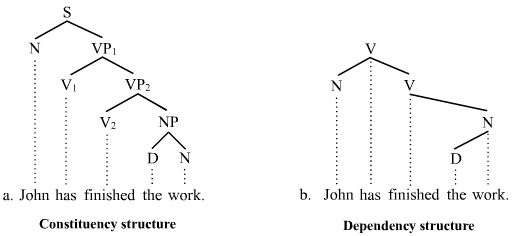
\includegraphics[width=0.7\textwidth]{figures/Johnhasfinishedthework}
	\caption{Parses of the sentence \textit{"John has finished the work"} \cite{parsers}}
	\label{fig:johnfinished}
\end{figure*}
%-------------------------------------------------------------
\section{Objectives}
The main focus of this study is computational semantics. My research includes building explicit representations of natural language semantics, because in today's state-of-the art systems for popular semantics tasks such as measuring semantic similarity or machine comprehension, they are rarely present. Virtually all systems
competing at popular challenges (e.g. \cite{Cer:2017,Collados:2017}) rely on word embeddings as the sole representation of word meaning. Recently \cite{Recski:2016c} has presented a method using graphical representations of natural language text that improved over the state-of-the art on the task of
measuring semantic similarity of pairs of English words. In this thesis
I use similar graphs as simple but powerful tools for measuring textual
entailment. My task includes defining new inference rules and methods for measuring graph similarities, and building an online available service for building graphs highly automatically, giving us a tool for building strong baseline methods. My work was based upon measuring our models through various semantic tasks such as Knowledge base population or the state-of-the art system on the 2018 Semeval Task \textit{Machine comprehension using commonsense knowledge}.

\section{Results}
We present a novel method for recognizing entailment using semantic
graphs and apply it to the tasks:
\begin{itemize}
    \item Knowledge base population task (KBP)
    \item 2017 RepEval task on Natural language inference (NLI)
    \item 2018 Semeval task on Machine
    Comprehension (MC).
\end{itemize}
First we present a highly automated process of building concept graphs from raw text building a microservice.
For the tasks I used the automatically built Concept graphs using the REST-API I defined based on the semantic parsing system \texttt{4lang} \cite{Recski:2016d}.
In the case of the KBP task I present a set of pilot experiments for augmenting a generic, open-domain 
knowledge base using a graph-based lexical ontology of English and simple
inference rules yielding millions of new facts with high
accuracy (over 90\% according to manual evaluation), the result was already presented in \cite{Kovacs:2018}.
For the NLI and MC task a strong baseline is presented using only concept graphs achieving accuracy scores of $67.5\%$ and $68.3\%$ respectively.
Followed by an enhancement of a state-of-the art system
\cite{Wang:2018}, where we proceeded to use the metric underlying our baseline as an additional feature. Preliminary results suggest that these features achieve a .5 percentage point improvement over the original system. This result was the output of the combined work with G\'emes Kinga presented in \cite{Kovacs:2018b}.

\section{References}
The code of the system is available on Github\footnote{\url{https://github.com/adaamko/4lang}}. The code was implemented by the author of this paper based upon the \textbf{4lang} system.

\section{Structure}
The structure of the paper is the following:
\begin{itemize}
	\item \textbf{Chapter \ref{chap:Introdu}} describes the short history and motivation of the NLP applications, it also gives a short summary about the objectives of the thesis, and the results.
	\item \textbf{Chapter \ref{chap:semanticparsing}} gives a short introduction into the field of semantic parsing, and semantic models in general. It briefly explains the semantic parsing system \textbf{4lang}, and my process of automating the building of concept graphs, and the newly defined inference methods
	\item \textbf{Chapter \ref{chap:comprehension}} describes the baseline approach to the Machine Comprehension task, which achieved an accuracy score of $68.3\%$.
	\item \textbf{Chapter \ref{chap:deep}} gives an introduction into deep learning, focusing on the NLP tasks.
	\item \textbf{Chapter \ref{chap:yuanfudao}} presents our experiments with the state-of-the art system \textbf{Yuanfudao}. Our preliminary results show a .5 percent improvement over the original system.
	\item \textbf{Chapter \ref{chap:future}} summarizes our contributions and describes our ongoing/future work. It briefly discusses our plans for the follow-up, that was beyond the scope of this work.
\end{itemize}

\section{Division of labour}
This project was a product of the combined work of Kov\'acs \'Ad\'am and G\'emes Kinga. Kov\'acs \'Ad\'am was responsible for building the service to automate the process of building concept graphs (online demo available at \url{http://4lang.hlt.bme.hu}), and was mostly working on the baseline methods and defining new inference rules and metrics for the given tasks. G\'emes Kinga's main work involved applying the baseline to the state-of-the-art system Yuanfudao \cite{Wang:2018}\footnote{\url{https://github.com/GKingA/commonsense-rc}} and experiments with IRTGs briefly described in Chapter \ref{chap:future}\footnote{\url{https://github.com/GKingA/irtg}}.
%----------------------------------------------------------------------------
\chapter{Semantic models and parsing}
\label{chap:semanticparsing}
%----------------------------------------------------------------------------

In this chapter I first introduce applications, that use semantic models as an essential knowledge for their process. After, the theory and problems of semantic representation are discussed, and I briefly present the upsides and downsides of such representations. After that we go into details about distributional and graph based models, introducing the semantic parsing system \textbf{4lang}, which is the main focus of our work. Finally, our micro-services are discussed, built around the parser to highly automate the process of building concept graphs from raw input. An easy example of their usage is shown as well.

When we use the word semantics, we usually refer to the interpretation of a linguistics unit (e.g. words, phrases, sentences, or whole texts) within the boundaries of a certain context. In many scientific fields e.g. philosophy, logic or biology the study of semantics is a highly researched task. While many NLP tasks like syntactic parsing, part-of-speech tagging, or even machine translation can be ignorant of the meaning of units, of what information they hold, there are also many other tasks that rely heavily on semantics.

Some examples, where semantic analysis is unavoidable:
\begin{itemize}
	\item \textbf{Question answering} is the process of generating meaningful answers to the user's question, using some kind of knowledge. It might be considered one of the oldest tasks in NLP or in AI in general with machine translation. With the recent rise of products like Siri, Alexa, or Watson, it is still one of the most researched area.
	\item \textbf{Recognizing entailment} is whether a statement implies another or not, it is closely connected to \textbf{machine comprehension}, which is the main focus of our work.
	\item \textbf{Chatbots} are systems, that somewhat can simulate the conversation of humans.
	\item \textbf{Sentiment analysis} is the task of understanding the opinion about a subject. Usually can be considered as a classification problem, where in the simplest case two class, "\textit{negative}" and "\textit{positive}" is given. More complex version of the task is also present, where the detection of the target of the opinion is also the part of the problem. There are solutions for the problem with hand-crafted rules and machine learning algorithms as well.  
\end{itemize}

For modeling the meaning of linguistic units, choosing an appropriate representation of our model is needed. While for syntactic analysis widely accepted concepts and ideas (e.g. dependency tree, phrase structure trees) of such representation are already in use, for a semantic model it still remained a challenging task. Even answering the question \textit{"What is a semantic representation?"} is not well defined, and mostly decided by the nature of our task. The units of a semantic model are also not globally decided (word, phrase or a sentence?).

Finding an absolute representation of semantics knowledge is among the most difficult task in Artificial Intelligence (AI). While we are yet to find a representation that has no downside, various experimental models are present, that are applicable for certain domains, but are problematic in other scenarios. So before choosing one, we need to take into account the limitations of each choice. 


Representation of semantic knowledge with logical expressions (e.g. zero-order logic, prepositional logic) exists, and although many companies still rely on hand-crafted rules as a knowledge representation, they are very unpractical and have serious problems with scalability and automation. Distributional models have risen in popularity in recent years, where meaning is represented with multi-dimensional vectors. While vector based models can give us a uniform representation, they mostly lack interpretability in a way that we never really know what happens inside these models. Another issue is the choice of the dimension. Many algorithms exist for reducing the dimension of such vectors to a fixed number, but determining the correct length can be difficult. Rare words are a big issue as well, if a word in the training data is rarely present, distributional models will fail to handle them correctly.

On the other hand, graph based solutions have high level of interpretability, and handling rare words is one of their biggest advantage. But automating the process of building graphs is a challenging task, and using them as a sole solution for a semantic parsing task in most cases would come short, but in hybrid systems they make up for the weaknesses other models have.

 In the next sections I will briefly discuss graph based models and distributional models, and because both of them have their merits, it is necessary to know the strengths and weaknesses of each one. My work focuses around graph based solutions.

\section{Distributional model}
In the field of natural language processing one way of encoding semantic meaning is to use distributional models. They model semantic meaning as real-valued vectors. These vectors need to be constructed from a training data, and we can calculate similarity as cosine distance between the vectors.

Let's have a look at these two sentences \textit{"The cat is walking in the bedroom"} and \textit{"A dog was running in a room"}. Words \textit{"dog"} and \textit{"cat"} have a similar semantic meaning, so if they are represented by vectors, and their cosine distance from each other is small, then we can vary the sentences \textit{"The dog is walking in the bedroom"} and \textit{"A cat was running in a room"} \cite{Bengio:2003}. These models take surrounding words into account and their goal is to obtain the meaning of the target word from their surroundings\cite{Jurafsky:2018}, and because \textit{"dog"} and \textit{"cat"} are close in vector space, they most likely will appear in the same context. This intuition helps us generalize sentences. These meanings are represented by vectors, called embeddings. One of the first models built around these intuitions were introduced in \cite{Bengio:2003}. 

These word embeddings are used in basically all state-of-the art systems related to natural language processing applications. Mikolov \cite{Mikolov:2013c} showed that word embeddings can be applied for vector operations, like addition or subtraction, and these operations often result in meaningful representation. If we have example words "\textit{King}", "\textit{Man}", "\textit{Woman}", then the vector("King") - vector("Man") + vector("Woman") \ref{fig:vecs} will most likely result in vector that is close to vector("Queen") in the embedding space.

 While the usage of word embeddings brought an important breakthrough in modeling word meaning, applying them for bigger linguistics units like phrases, sentences or even whole text remained a difficult challenge even for nowadays. One of the biggest reasons for this is the additive aspect of these models: if we model A B C expression with vector v(A) + v(B) + v(C), then we represent "John killed Bill" and "Bill killed John" sentences in the same way. 

\begin{figure*}[h!]
	\centering
	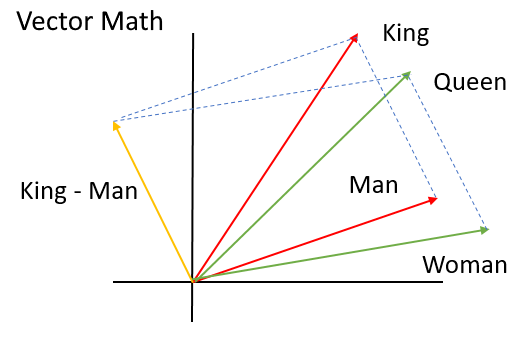
\includegraphics[width=0.7\textwidth]{figures/vecs}
	\caption{Vector addition example \cite{embeddings}}
	\label{fig:vecs}
\end{figure*}

The other issue is that we know very little about the structure of a multi-dimensional real-value vectors (for embeddings it can be from 300 up to 1000 dimension), so this makes it very hard to understand their structure, and exactly in what scenario they work, and the reason when they don't. So while most state-of-the art systems use word embeddings as a sole representation of meaning, and while it can be useful to encode meaning as vectors, so it can create connection from language specific and non-language specific data, we cannot deny the importance of having other semantics representations, such as graph-based ones. 

In the majority of my work, I researched graph-based solutions, where I model the meaning of linguistics unit with graphs, and the whole process can be defined with graph transformations. Next, I will briefly introduce graph based formalism starting with Abstract Meaning Representations (AMR) followed by the introduction of the \textbf{4lang} formalism, which will be the focus of the thesis, and I will go into details in the next section.

\section{Abstract Meaning Representations}
Abstract Meaning Representation (AMR) was introduced by Banarescu\cite{Banarescu:2013} for representing the meaning of linguistic structures. They represent meaning as directed acyclic graphs (DAGs), that can be used to capture the meaning of whole sentences. In the past few years, AMR related works have appeared e.g. parsing applications, or annotated corpuses \cite{Banarescu:2013, OGorman2018AMRBT, DAC:2017}.

Nodes of AMR graphs can be represented various ways. Each node in the graph represents a semantic concept \cite{AMR:2015}, that can be either an English word, or frameset from PropBank \cite{Palmer:2005}, essentially used for abstraction. The framesets are English verbs. The AMR introduced these variables for entities, events, properties, and states. An AMR can be converted to multiple formats:
\begin{itemize}
	\item Logic format
	\item AMR format
	\item Graph format
	
	These formats can be seen on Figure \ref{fig:amr} for sentence \textit{"the boy wants to go"}, and the corresponding 4lang representation on Figure \ref{fig:4langboy}.
	
\end{itemize}

\begin{figure*}[h!]
	\centering
	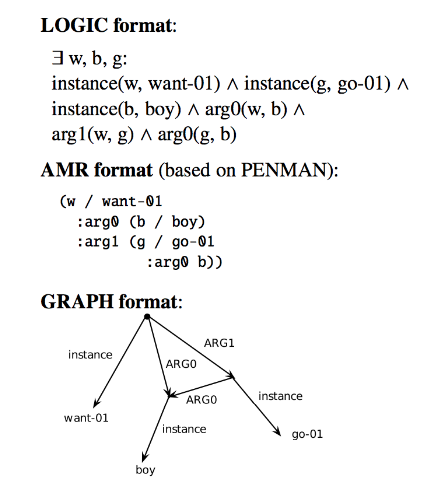
\includegraphics[height=0.4\textwidth]{figures/amr}
	\caption{Example sentence and representations \cite{Palmer:2005}}
	\label{fig:amr}
\end{figure*}

In this paper I use the semantic parser \textbf{4lang} \cite{Recski:2018}, and unlike \textbf{4lang}, AMR handles wider range of phenomenas, mostly typical of English. AMR's usage is mostly biased towards English \cite{Palmer:2005}, while 4lang can be configured to handle multiple languages.

\begin{figure*}[h!]
	\centering
	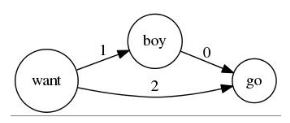
\includegraphics[width=0.3\textwidth]{figures/4langboy}
	\caption{Example sentence and representations in 4lang}
	\label{fig:4langboy}
\end{figure*}

In the next section, I will go into details about the \textbf{4lang} formalism, and the parser itself. After that I will describe our method of measuring similarities between semantic graphs, and its usage on semantic related tasks.

%----------------------------------------------------------------------------
\section{4lang}
\label{sec:4lang}
%---
The \textbf{4lang} system is in the main focus of my work, this section discussed the formalism and possible applications. \textbf{4lang} also means the manually built dictionary of mapping more than 2000 words to graphs, this is described in \cite{Kornai:2013}. After discussing the main formalism of \textbf{4lang}, I will demonstrate my highly automated process of building concept graphs, that was achieved by wrapping \textbf{4lang} functionality in micro-services building a REST-API, followed by our baseline for the machine comprehension task.

\subsection{The formalism}
The \texttt{4lang} system of semantic representation \cite{Kornai:2015a}
represents the meaning of linguistic units (both words and phrases)
as directed graphs of syntax-independent concepts. Every node of a \textbf{4lang} graph is a concept, which means that they are not taken as words, and they don't have any grammatical functions, like part-of-speech, voice, tense, etc.\cite{Recski:2016}.
Since these concepts have no grammatical attributes and no event structure, e.g.
the phrases \textit{water freezes} and \textit{frozen water} would both be
represented as \textit{water}~$\xrightarrow0$~\textit{freeze}. This also means that 4lang defines a many-to-one relation between the words and concepts. 

\textbf{4lang} formalism defines three types of edges:
\begin{itemize}
	\item \textbf{The 0-edge} represent represent attribution (\texttt{dog
		$\xrightarrow0$ large}), hypernymy (\texttt{dog $\xrightarrow0$ mammal}) and unary predication (\texttt{dog  $\xrightarrow0$ bark})
	\item \textbf{1- and 2-edges} those representing binary relations are connected to their arguments
	via edges labeled \texttt{1} and \texttt{2}, e.g \texttt{cat $\xleftarrow1$ catch $\xrightarrow2$ mouse}. Binaries that are shown with uppercase are binaries that must have two outgoing edges as shown in Figure \ref{fig:4langbin}. If we look at the sentence \textit{"Kinga broke Adam's bike"}, and the corresponding graph shown in Figure \ref{fig:4langbin}, if the 0-connection wouldn't be present between \textit{Kinga} $\xrightarrow0$ break, that would mean we consider that the relationship depend on whether the object of breaking is established or not. So in \textbf{4lang} the connection of 0-edge is present between a subject and a predicate regardless of the other arguments.
\end{itemize}

\begin{figure*}[h]
	\centering
	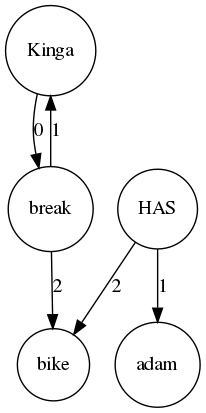
\includegraphics[height=0.5\textwidth]{figures/binary4lang}
	\caption{4lang with binaries}
	\label{fig:4langbin}
\end{figure*}

The example in
Figure~\ref{fig:bird} shows the \texttt{4lang} definition of the
concept \texttt{bird}. This definition was built manually, as part of
the \texttt{4lang} dictionary \cite{Kornai:2013}, but similar
definitions have been created automatically from definitions of
monolingual dictionaries such as Longman, using the
\texttt{dict\_to\_4lang} tool \cite{Recski:2016d}.

The open-source \textbf{4lang} pipeline\footnote{\url{https://github.com/kornai/4lang}}
contains tools for generating
directed graphs from raw text by mapping dependency edges in the output of the
Stanford parser \cite{deMarneffe:2006} to \texttt{4lang} subgraphs over
concepts corresponding to each word of the original sentence. The Stanford parser builds a dependency tree from the raw text that captures the syntactical relations between the linguistics units. \textbf{4lang} graph construction involves mapping from these relations to \textbf{4lang} semantics graphs, assigning the dependencies to \textbf{4lang} subgraphs. The mapping is presented in Table \ref{table:mapping}, and an example is shown for sentence \textit{"I like swimming"} in Figure \ref{fig:swimmingdep}, where we can see the dependency tree coming out of the Stanford parser, and the corresponding 4lang graph is present in Figure \ref{fig:swimming}, where the mapping from the dependency tree to \textbf{4lang} graph is done. 

\begin{table}
	\centering
	%\small
	\begin{tabular}{lc}
		\toprule
		Dependency & Edge \\
		\midrule
		amod & \multirow{7}{*}{\edge{$w_1$}{0}{$w_2$}} \\
		advmod & \\
		npadvmod & \\
		acomp & \\
		dep & \\
		num & \\
		prt & \\
		\midrule
		nsubj & \multirow{4}{*}{\twoedges{$w_1$}{1}{0}{$w_2$}} \\
		csubj & \\
		xsubj & \\
		agent & \\
		\midrule
		dobj & \multirow{6}{*}{\edge{$w_1$}{2}{$w_2$}} \\
		pobj & \\
		nsubjpass & \\
		csubjpass & \\
		pcomp & \\ 
		xcomp & \\
		\midrule
		appos & \twoedges{$w_1$}{0}{0}{$w_2$} \\
		\midrule
		poss & \multirow{2}{*}{$w_2\xleftarrow1$ \texttt{HAS} $\xrightarrow2w_1$} \\
		prep\_of & \\
		\midrule
		tmod & $w_1\xleftarrow1$ \texttt{AT} $\xrightarrow2w_2$ \\
		\midrule
		prep\_with & $w_1\xleftarrow1$ \texttt{INSTRUMENT} $\xrightarrow2w_2$ \\
		\midrule
		prep\_without & $w_1\xleftarrow1$ \texttt{LACK} $\xrightarrow2w_2$ \\
		\midrule
		prep\_P & $w_1\xleftarrow1$ \texttt{P} $\xrightarrow2w_2$ \\
		\bottomrule
	\end{tabular}
	\caption{Mapping from Stanford dependency relations to \textbf{4lang} subgraphs \cite[p. 12.]{Recski:2018}.}
	\label{table:mapping}
\end{table}

\begin{figure*}[h]
	\centering
	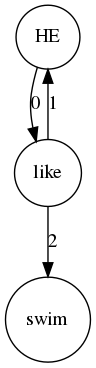
\includegraphics[height=0.5\textwidth]{figures/swimming}
	\caption{4lang example of a sentence}
	\label{fig:swimming}
\end{figure*}

\begin{figure*}[h]
	\centering
	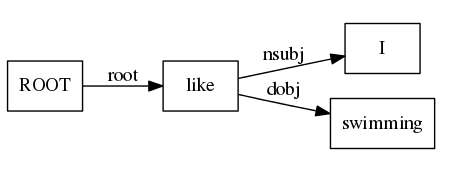
\includegraphics[width=0.5\textwidth]{figures/swimmingdep}
	\caption{Stanford example of a sentence}
	\label{fig:swimmingdep}
\end{figure*}


\subsection{Expansion}
Optionally, the \texttt{4lang} system allows us to \textit{expand}
graphs, a process which unifies the graph with the definition graphs of
each concept. The implementation is written in the \textbf{dict\_to\_4lang} module, that extends the functionality of the discussed \textbf{text\_to\_4lang} pipeline with dictionaries. \textbf{4lang} takes advantage of this, and implements the expansion step, which is essentially joining the definitions graphs to the main graph. This allows us to build a larger graph, that contains more information, and allows us to model the text better by simply adding the definition of words.

Let us look at the example sentence \textit{"My poor wife"}, that results the graph shown in Figure \ref{fig:mypoor}. Looking at the definition of the word \textit{poor}: \textit{having very little money and not many possessions}, we can build a definition graph and essentially join the two graphs together. This can result us a better model if we are ready to take word definitions into account, and with this method we can have higher similarities between graphs whose sentences are also similar \footnote{Of course not every interpretation of \textit{"poor"} is related to money. It requires a higher level mechanism to handle these kind of occurrences, see more in \cite{Kornai:2018}.}. Doing this for every word in the sentence resulting in a merged graph Figure \ref{fig:mypoorexpanded}. If we look at the graph, it is clear that the expanded graph gives us much more accurate context and definition. My work was built around the expanded graph, and enhancing it with inference rules. We will see that how better it actually performs on a real task. This will be the main topic of Chapter \ref{nli}.

\begin{figure}
	\centering
	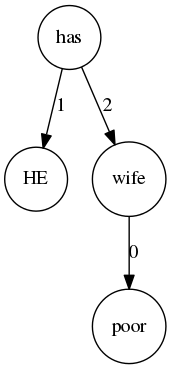
\includegraphics[scale=0.5]{figures/mypoor}
	\caption{4lang definition of sentence \textit{"My poor wife"}.}
	\label{fig:mypoor}
\end{figure}

\begin{figure}
	\centering
	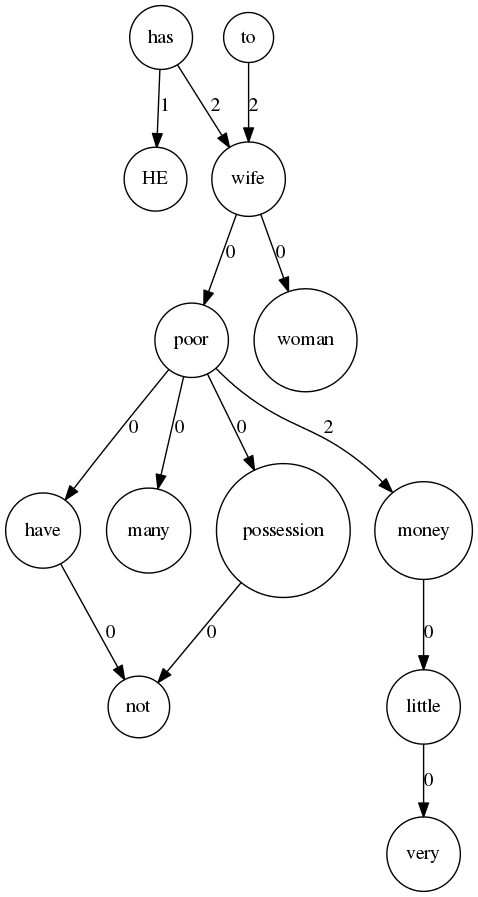
\includegraphics[scale=0.5]{figures/mypoorexpanded}
	\caption{4lang definition of expanded sentence \textit{"My poor wife"}.}
	\label{fig:mypoorexpanded}
\end{figure}


\subsection{The service}
At the beginning of my research I put a high emphasis on generating graphs from raw text with a highly automated method, so besides being an open-source software library, one of my contribution consists of the accessibility of \texttt{4lang} via a public
REST API at \url{http://hlt.bme.hu/4lang}. I used the python language for implementing the service, and for the framework I used the flask\footnote{http://flask.pocoo.org/} package. The service generates input for the \texttt{text\_to\_4lang} module from the raw text input, then after processing it, returns a graph in \textbf{networkx multigraph}\footnote{\url{https://networkx.github.io/documentation/networkx-1.9.1/reference/classes.multigraph.html}} format to make it easy to visualize it on essentially any client side. Online demo of the service is available at \url{http://4lang.hlt.bme.hu}. 
The process is presented in Example \ref{lst:code}.
\begin{center}
	\begin{lstlisting}[caption={Demonstration of the service in python language.},language=python, label={lst:code}]
sentence = "I like micro-services." 
data = {'sentence':   sentence}
data_json = json.dumps(data)
payload = {'json_payload': data_json}
headers = {'Content-type': 'application/json', 'Accept': 'text/plain'}
r = requests.post("http://hlt.bme.hu/4lang/sendef", 
data=data_json, headers=headers)
s_machines = r.json()['sentence']
\end{lstlisting}
\end{center}


The generated graph can be seen in Figure \ref{fig:service}. The code of the service is publicly available on Github\footnote{\url{https://github.com/adaamko/4lang}}. We can generate graphs with raw text by calling the service. Currently my service has multiple endpoints, with each of them representing different methods.
If you are only interested in processing a single sentence, the following endpoints are available:

\begin{figure}[!htb]
	\centering
	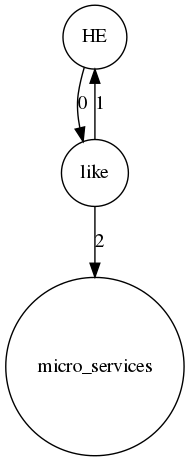
\includegraphics[scale=0.4]{figures/service}
	\caption{4lang definition of sentence \textit{"I like micro-services"}.}
	\label{fig:service}
\end{figure}

\begin{itemize}
	\item \textbf{/sendef} - Returns the graphs built from the sentence.
	\item \textbf{/senexp} - Returns the graphs, where the word's definition has been added to the graph.
	\item \textbf{/senabs} - Calling this function, with the help of simple inference rules, we can build more abstract graph that in certain scenarios can capture meaning in a different way than the expand function does. While the functionality is already implemented, it is yet to reach the results of the expansion method, so it can be described as a more of a future work, we will explain the method in Chapter \ref{chap:nli}.
\end{itemize}
You can get a word's definition by calling the defined endpoint:
\begin{itemize}
	\item \textbf{/definition} - Returns the graphs built from the word's definition.
\end{itemize}
For the machine comprehension task we defined a dedicated endpoint:
\begin{itemize}
	\item \textbf{/rally} - Returns a merged graph, where we merge a question sentence with an answer sentence. The main goal of this endpoint is that we can get a graph that can be explicitly compared with graph built from the passage text (it will be explained in Chapter \ref{chap:comprehension } concretely). 
\end{itemize}


\begin{figure}[!htb]
	\centering
	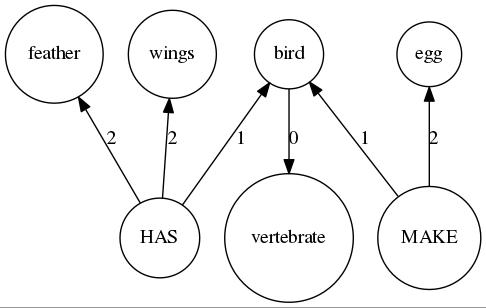
\includegraphics[scale=0.5]{figures/bird}
	\caption{4lang definition of \texttt{bird}.}
	\label{fig:bird}
\end{figure}

Graphs generated by the \texttt{4lang} parser have previously been used
successfully in measuring semantic similarity. The current state of the
art system on the \texttt{SimLex-999} benchmark \cite{Hill:2014a}
outperforms previous top systems by utilizing a simple similarity metric
between \texttt{4lang} definitions of pairs of English words
\cite{Recski:2016c}, this was the main idea of trying it in a different task with a different state-of-the-art system.

In the next chapter, I will briefly discuss the main challenges we chose for evaluation, mainly the task of KBP. After, I will introduce our baselines methods for solving the NLI and MC tasks using our micro-service for automatically building concept graphs. Finally I will present our mutual work, where we made it applicable to an already working system.
\chapter{Knowledge Base Population}
\label{chap:kbp}

Since my methods can only be evaluated through well defined tasks, I chose multiple challenges where measuring the accuracy of my models can be verified. This chapter includes the task of Knowledge base population which goal is to discover facts about entities and augment a knowledge base with these facts. In this challenge we achieved a high accuracy of generating millions of new facts only using simple inference rules. After that, in the next Chapter, I will discuss my experiments with Natural language inference, where I will introduce my method of measuring support score of the concept graphs, and defining new inference rules to enhance the expansion method, generating a more abstract version. Next my baseline to the NLI task is discussed, followed by the review of my problems with the \textit{MultiNLI} dataset \footnote{\url{https://www.nyu.edu/projects/bowman/multinli/}}. Finally I explain the machine comprehension challenge, and I will introduce my baseline method for solving it, using my micro-service for automatically building concept graphs. After that I will present how we made it possible to integrate it to an already working system that uses deep learning algorithms.

%----------------------------------------------------------------------------
\section{Introduction} 
The first task I chose to evaluate my models on was the Knowledge base population challenge. Here I present a set of pilot experiments for augmenting a generic, open-domain 
knowledge base using a graph-based lexical ontology of English and simple
inference rules. The WikiData knowledge-base contains facts encoded as relation
triplets, such as author(George Orwell, 1984), based on which naive
speakers can easily establish additional facts such as that George Orwell is a
person and 1984 is some written work, most likely a book. To automate this type
of inference we need models of lexical semantics that are more explicit than
the distributional models commonly used in computational semantics. For this I used my REST-API built on the \textbf{4lang} formalism to automatically build concept graphs. The representation of "author" will likely contain edges
corresponding to facts such as \texttt{IS\_A(author, person)} and
\texttt{write(author, book)}.
I define simple templates that use these representations for inference over
WiktData facts. My method yields millions of new facts with high
accuracy (over 90\% according to manual evaluation)

\section{Background}
\texttt{WikiData}\footnote{\url{https://www.wikidata.org/}}
is a public domain knowledge base containing
attribute-value type information about more than 30 million entities.
For each entity, WikiData contains pairs of \textit{properties}
(attribute) and \textit{values}, which may contain pointers to other
entities. In case of the entity \texttt{1984}, the value of the property
\texttt{author} is \texttt{George\_Orwell}. An alternative
representation of the dataset is in the form of relational triplets,
this would represent the above fact as a single binary relation
\texttt{author(George\_Orwell, 1984)}. I use This latter representation
when processing WikiData and use the \textbf{4lang} service to process this set of
definition graphs when performing inference over WikiData triplets. These triplets can be generated from the \textit{json} format of the dataset, which is online accessible. The first step I had to take was to preprocess the raw dataset to obtain the triplets format. For this I used python language as well.

\section{Method}
Two simple patterns were implemented for performing inference using
\texttt{WikiData}
triplets and \texttt{4lang} definitions. Given the triplet
\texttt{author(George\_Orwell, 1984)} and the definition graph
of \texttt{author} in Figure~\ref{fig:author}, it should be doable to
infer all edges in the graph in Figure~\ref{fig:orwell_inf}. This
requires an implementation of two patterns. Given a triplet $R(X, Y)$, I
first found nodes in the \texttt{4lang} definition of $R$ that are connected
to $R$ by an outgoing 0-edge (e.g. \texttt{author} $\xrightarrow0$
\texttt{write}) and assumed that each of these 0-relations holds for $X$.
The second inference I would like to make is \texttt{1984}~$\xrightarrow0$~book
based on the \texttt{4lang} edge \texttt{write} $\xrightarrow2$ book. To this end
I implemented the rule that if for any relation $R$ and concepts $B$ and $C$
I found $R \xrightarrow0 B \xrightarrow2 C$, then for each triplet $R(X, Y)$ I
added the edge $Y \xrightarrow0 C$. 

An issue I encountered early concerns words with multiple outgoing
0-edges in their definition graph. Often, this is the result of a
dictionary definition that lists several categories that the concept may
belong to, e.g. the definition of \texttt{employer} is \textit{a person,
	company, or organization that employs people}. In case of a triplet such
as \texttt{employer(CIA, Mike\_Pompeo)}, the incorrect inference
\texttt{CIA} $\xrightarrow0$ \texttt{person} would be made. Special treatment for such
constructions by \textbf{4lang} and/or my system might handle these cases and
make the inference that the CIA is either a person, a company, or an
organization, but for the purpose of the present experiment I decided
to discard all \texttt{WikiData} relations whose \texttt{4lang}
definition contains more than one outgoing 0-edge.

Other issues are caused by meaningless or erroneous 0-connections in 4lang graphs
that are ultimately limitations of the method used by the \texttt{dict\_to\_4lang}
system to build these graphs from natural language definitions. The process involves parsing
the definitions with a state-of-the-art dependency parser and mapping grammatical
relations between pairs of words to configurations of \texttt{4lang} edges.
In case of a definition such as \textbf{flag:}
\textit{piece of cloth with a coloured pattern or picture on it that represents
	a country}, the definition graph will contain the edge
\texttt{flag} $\xrightarrow0$ \texttt{piece}. This information
is obviously not informative (to say the least), we consider it an error
when evaluating my system.
To make a correct inference about flags similar to those in our previous example,
a system would need to learn something along the lines of
``\textit{piece of X} $\xrightarrow0$ \texttt{X}'', which is beyond the scope of
the current thesis. 
A final common source of false facts concerns words that are used in WikiData
in a very different sense than the one defined by the Longman dictionary, the source
of \texttt{4lang} definitions. One example is the outdated definition of
\texttt{developer}: \textit{a person or company that makes money by buying land
	and then building houses, factories etc on it}, which causes our method to erroneously
infer that developers are companies.

\begin{figure}
	\centering
	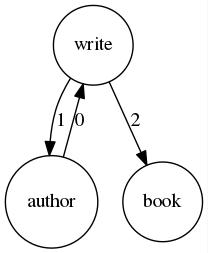
\includegraphics[scale=0.5]{figures/author.jpg}
	\caption{4lang definition of \texttt{author}.}
	\label{fig:author}
\end{figure}

\begin{figure}
	\centering
	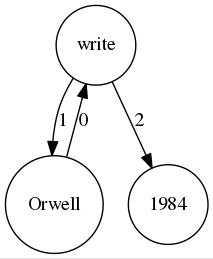
\includegraphics[scale=0.5]{figures/orwell_inf.jpg}
	\caption{4lang graph produced from WikiData triplet
		\texttt{author(George\_Orwell, 1984)}.}
	\label{fig:orwell_inf}
\end{figure}

\subsection{Evaluation}

In the WikiData dataset first I counted the triplets. I found 86.3 million triplets using 893 unique predicates.
I started our experiment by preprocessing WikiData to discard fragmentary data
(triplets with empty positions) and multi-word predicates that do not lend themselves
to the simple methods described in the previous section. This was made by python code, and is available on github \footnote{\url{https://github.com/adaamko/4lang}}.
After these steps the dataset consisted of 195 predicates and 19.6 million triplets,
out of which the first inference pattern was applicable to 108 predicates
(covering 9.2 million triplets), the second to 27 predicates (covering 1.4 million triplets).
After an initial examination of the output I decided to discard further subsets
of predicates: I applied our patterns to predicated whose definition graphs had exactly one outgoing
0- or 2-edge and no incoming edges. This step resulted in a considerable increase in
overall accuracy. After these steps I proceeded to apply our two patterns: the first one was
now applicable to 84 predicates (8.2 million triplets), the second to 25 predicates (0.8 million triplets).
This relatively small number of unique predicates allowed to inspect all of them manually and estimate the quality of all newly
extracted facts: if we find that for some predicate, e.g. \texttt{father}, I
have made inferences based on the template ``$X \xrightarrow0$ \texttt{father}
implies $X \xrightarrow0$ \texttt{male}'', it assumes that each fact inferred
using this template is correct, while for erroneous templates I assume that
each extracted fact is false. Figures are shown in Table~\ref{table:results}.
Note that our evaluation
was strict in the sense that we judged incorrect all non-informative edges, e.g.
$X~\xrightarrow0$~\texttt{something}.

\begin{table}
	\centering
	\begin{tabular}{lrrr}
		& 1-pattern & 2-pattern & total\\
		predicates  & 84 & 25 & 109 \\
		correct     & 55 & 17 & 72 \\
		new facts   & 8.2 million & 0.83 million & 9 million \\
		correct     & 7.6 million & 0.74 million & 8.3 million \\ 
		accuracy    & 0.92 & 0.89 & 0.92
	\end{tabular}
	\caption{Evaluation results}
	\label{table:results}
\end{table}

This pilot system presented here used simple pattern-based
methods for combining facts from a knowledge base with linguistic knowledge
represented in a lexical ontology. We believe
the significance of this experiment lies not in its yield of millions of high-quality
facts with which a knowledge base might be extended, but in its demonstration
that inference based on linguistic knowledge is a powerful
method for enriching any natural language data. In the next chapter I will discuss the NLI challenge, and my methods of measuring similarity between concept graphs.
\chapter{Natural Language Inference}
\label{chap:nli}

The NLI task is meant to evaluate language understanding. 
For most of the NLP tasks we are in big need of understanding entailment. Most of the part however we lacked the resources to measure machine learning methods correctly on this task. Stanford addressed this issue by introducing the Natural Language Inference corpus \footnote{\url{https://nlp.stanford.edu/projects/snli/}}, which is freely available collection of labeled sentence pairs, and were labeled by humans. In this chapter I will present my experiments with the dataset. An example from the dataset can be explained through the sentences \textit{"A soccer game with multiple males" } and 
\textit{Some men are playing a sport.}, where the task is to determine if the second sentence \textit{entails} the first sentence or not. The first sentence is called the \textit{premise} and the second is \textit{hypothesis}.

\section{Method}
For the task I define a simple metric between pairs of \texttt{4lang} graphs that
we intend to use for measuring entailment between a premise and a
hypothesis. I shall define the degree to which some graph $G_1$
\textit{supports} another graph $G_2$ as the ratio of edges in $G_2$
that are also present in $G_1$:

\[ S(G_1, G_2) =\frac{|E(G_1)\cap E(G_2)|}{|E(G_2)|}\]

Two (directed) edges are identical if their source
and target nodes, and their labels are all identical. I found out that this metric can be used in the MC challenge as well demonstrated accurately in Chapter \ref{chap:comprehension}.

Let's have the following sentences:
\begin{itemize}
	\item My poor wife!
	\item I feel bad for my wife!
\end{itemize}
Then we can run our service tool to generate the graphs from the sentences. From these sentences we generate the graphs seen in Figure \ref{fig:mypoor} and Figure \ref{fig:ifeelbad}. From the sentences we can already have an anticipation that these sentences are very similar, so the hypothesis sentence will be an entailment. So if we are ready to make an assumption, that an inference corresponds with the similarity of the graph's edges, than the graphs identify us that this is indeed an entailment. This simple method works for a lot of examples, but if we want higher accuracy, we need to define finer techniques. This is where the definitions of the words come into play. If we want higher accuracy, we need to take word definitions into account, building expanded graphs discussed in Chapter \ref{chap:semanticparsing}. With this method higher similarities between graph whose sentences are also similar can be achieved.

The experiments was run with the default and with the expanded methods as well, setting a threshold value, above what we consider \textit{entailment}. For the default method the results can be seen in Figure \ref{fig:nlidefault} and for the expanded method it can be seen in Figure \ref{fig:nliexpanded}. In the figures the axis y represents how accurate our model is. We defined metrics precision, recal, f1\_score and accuracy. Our task was essentially a binary classification, so f1\_score is a good indicator of our model. The axis x represents the threshold value, above what score we consider \textbf{entailment}. It is the support score that was calculated using the defined metrics. We can see that the expand method gives us better result around 0.4 threshold value.

\begin{figure}
	\centering
	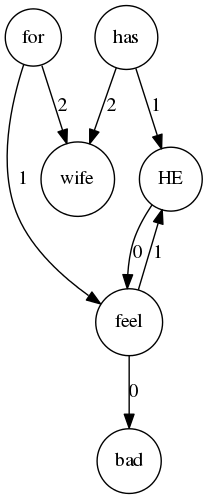
\includegraphics[scale=0.5]{figures/ifeelbad}
	\caption{4lang definition of sentence \textit{"I feel bad for my wife!"}.}
	\label{fig:ifeelbad}
\end{figure}

\begin{figure}
	\centering
	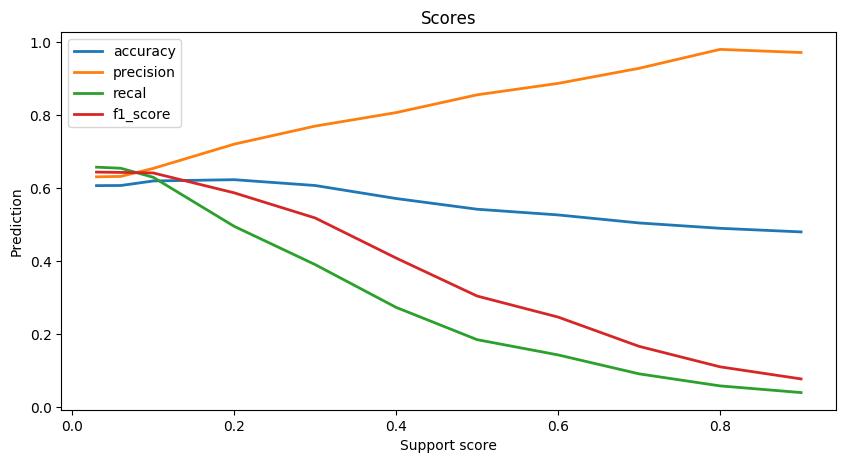
\includegraphics[scale=0.5]{figures/nlidefault}
	\caption{Baseline for the NLI task with the default method}
	\label{fig:nlidefault}
\end{figure}

\begin{figure}
	\centering
	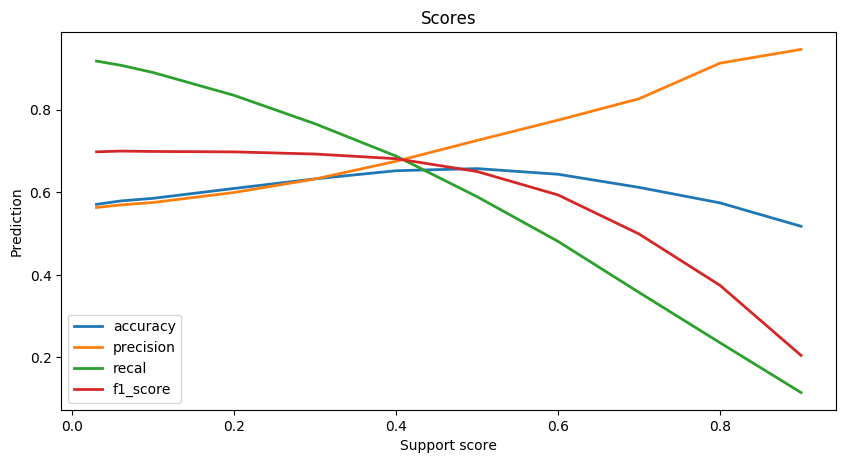
\includegraphics[scale=0.5]{figures/nliexpanded}
	\caption{Baseline for the NLI task with the expanded method}
	\label{fig:nliexpanded}
\end{figure}

\begin{figure}
	\centering
	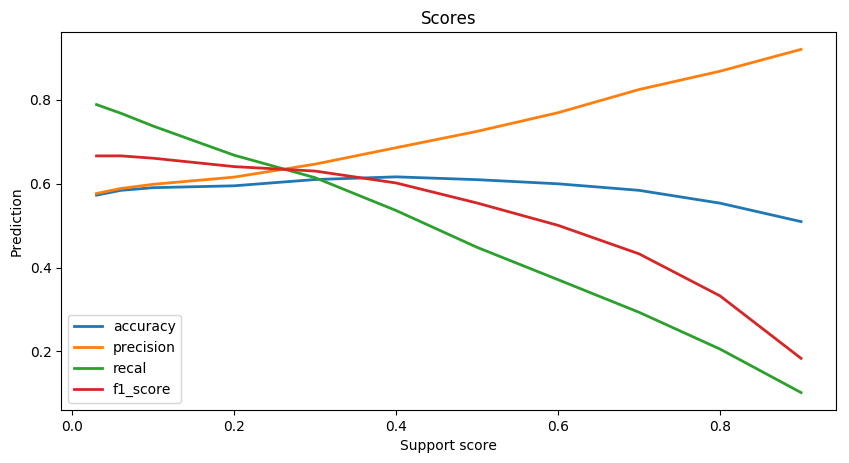
\includegraphics[scale=0.5]{figures/nliabstract}
	\caption{Baseline for the NLI task with the abstract method}
	\label{fig:nliabstract}
\end{figure}

\section{Abstract method}
We also have some experiments with defining new additional rules added to the \textbf{4lang} parser, that could potentially be giving us a more abstract and simpler definitions than the \textit{expansion} method. Let us look back the sentence "My poor wife" and the expanded graph shown in Figure \ref{fig:mypoorexpanded}. In this example if we look at the edge \textbf{wife $\xrightarrow0$ woman} we can make an assumptions, that native speakers can easily make using simple inference rules \cite{Kovacs:2018}. In our example, within the boundaries of the sentence we can use the concept \textbf{woman} instead of the concept \textbf{wife}. Using this simple rule we can reduce our graph to a simpler definition shown in Figure \ref{fig:mypoorabs}.

\begin{figure*}[h]
	\centering
	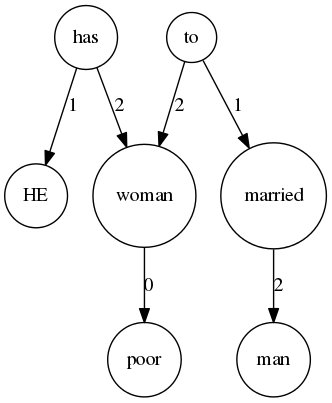
\includegraphics[scale=0.4]{figures/mypoorabs}
	\caption{Example of the \textit{"abstract"} method}
	\label{fig:mypoorabs}
\end{figure*}
Let's say we have a node machine in our graph, and it's definition graph, then we can define simple inference rules as follows:
\begin{itemize}
	\item If X $\xrightarrow0$ Y is present, then we can use Y instead of the X node.
	\item Y $\xrightarrow0$ X is present, then we can use Y instead of X node again.
	\item If we have Y $\xleftarrow1$ Z $\xrightarrow2$ X  both in the definition and the sentence graph, than we can connect every edge from X and Y from the definition graph to the sentence graph.
\end{itemize}
For the third rule, let's have the graph shown in Figure \ref{fig:thirdrule}, and say we have the definition of the concept increase in the graph in Figure \ref{fig:thirdrule2}, then by the rule number 3 we can add  additional edges to the price concept shown in Figure \ref{fig:thirdrule3}. Using these rules we also run our method for the dataset achieving results shown in Figure \ref{fig:nliabstract}. The result shows that the method cannot achieve the accuracy of the expand model for the dataset. But I believe that using the already defined simple inference rules, and adding some new ones as well could potentially define a model, where the captured meaning can exceed our results.


\begin{figure}
	\centering
	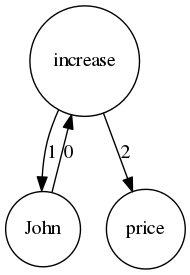
\includegraphics[scale=0.5]{figures/thirdrule1}
	\caption{4lang graph of "Jonh increased the price"}
	\label{fig:thirdrule}
\end{figure}

\begin{figure}
	\centering
	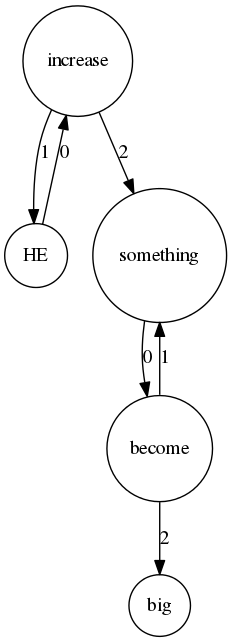
\includegraphics[scale=0.5]{figures/thirdrule2}
	\caption{4lang graph of the definition of "increase"}
	\label{fig:thirdrule2}
\end{figure}

\begin{figure}
	\centering
	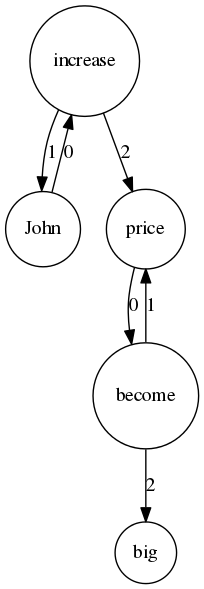
\includegraphics[scale=0.5]{figures/thirdrule3}
	\caption{Abstract graph}
	\label{fig:thirdrule3}
\end{figure}

Based on early findings I discovered using the abstract rules doesn't gives us better results, so in the MC task we used only \textit{expanded} \texttt{4lang} graphs (see
Section~\ref{sec:4lang}) for measuring support. 

\section{Problems}
I also found the dataset problematic for our methods, this gave me the intuition to move to the MC challenge. Few examples from the dataset, where my method yielded high support score, but the prediction was wrong:

\textbf{score}: 0.870967741935

\textbf{premise}: \textit{European Tour, takes place at Santo da Serra Golf Club.}

\textbf{hyp}: \textit{The European tour can be found at the Santo da Serra Golf Club.}
\newline

\textbf{score}: 0.864864864865

\textbf{premise}: \textit{Thorn and the Kal will help prepare the spikes.}

\textbf{hyp}: \textit{Thor and the Kal will help the others prepare the spikes. }
\newline

\textbf{score}: 0.851063829787

\textbf{premise}:  \textit{"Heard tell as you boys don't think th' war's clear over yet,"Fenner observed.}

\textbf{hyp}: \textit{Fenner heard in the bar that these boys don't think the war is over.}
\newline

\textbf{score}: 0.909090909091

\textbf{premise}: \textit{To many Madeirans who believe the Lady of Monte has carried them through troubled times, the pilgrimage is an obligation.}

\textbf{hyp}: \textit{Because the Lady of Monte is believed to have carried them through troubled times, Madeirans believe the pilgrimage is an obligation.}
\newline

Likewise some examples were found where our model didn't find any connection, nevertheless the label was entailment:

\textbf{score}: 0.0

\textbf{premise}: \textit{(Emphasis added.)}

\textbf{hyp}: \textit{The emphasis was added by the editor.}
\newline

\textbf{score}: 0.0

\textbf{premise}: \textit{From Beforethewars."}

\textbf{hyp}: \textit{From before the wars.}
\newline

\textbf{score}: 0.0

\textbf{premise}: \textit{Ten years, sir.}

\textbf{hyp}: \textit{About a decade, sir.}
\newline

We want to move towards a goal, where our model can handle simple, trivial situations, that humans find themselves in everyday. Nevertheless we believe that these cases would not be a good base for us to rely on.
In the next chapter I will give an introduction to the Machine comprehension task defining my baseline. After an introduction to the field of Deep learning is discussed, followed by it's integration to a state-of-the art system, achieving a 0.5 percent improvement.
\chapter{Machine Comprehension}
\label{chap:comprehension}
In this chapter a brief introduction to the machine comprehension task is given, followed by the application of our metric discussed in the previous chapter, that was defined for measuring similarity between concept graphs. After our baseline for the task presented.

The 2018 Semeval Task \textit{Machine comprehension using commonsense
	knowledge}\footnote{\url{https://competitions.codalab.org/competitions/17184}}
requires participants to train systems that can choose the
correct answer to simple multiple choice questions based on short
passages describing simple chains of events. Data for both training and
testing is extracted from the \texttt{MCScript} dataset
\cite{Ostermann:2018}. Some questions can only be
answered using commonsense knowledge, and are
explicitly labeled as such. For example, one passage might describe a
story of a gardener planting a tree, and one of the questions would
subsequently ask whether the gardener used his hands or a shovel to dig
a hole for the tree, even though the answer to this question is not
present in the passage. The top two systems, \texttt{HFL-RC}
\cite{Chen:2018} and
\texttt{Yuanfudao} \cite{Wang:2018} achieved accuracy scores of
$84.15\%$ and $83.95\%$ on the test data, respectively. In our experiments we used
semantic graphs to augment the \texttt{Yuanfudao} system, since its source
code is publicly
available\footnote{\url{https://github.com/intfloat/commonsense-rc}} and since it already employs successfully a
knowledge base representing semantic relationships among pairs of words.

\section{Comprehension, entailment, and knowledge bases}

In the next section we shall present a simple method for measuring
\textit{support}, the continuous counterpart of \textit{entailment},
based on graphical representations of meaning, and use this metric in a
baseline for machine comprehension and to improve a state of the art
MC system.
Although explicit representations of semantics are rarely used for this purpose,
in recent years there have been several attempts at leveraging lexical
ontologies in machine comprehension, and the approach of using textual
entailment as an intermediary task is also not new. \cite{Wang:2016}
achieves competitive results on the \texttt{MCTest} dataset
\cite{Richardson:2013} by generating
answer candidates and ranking them using a separate RTE system, which is
trained on the Stanford Natural Language Inference (SNLI) dataset
\cite{Bowman:2015}
but also relies on an explicit measure of lexical overlap between sentence
pairs. Other recent systems are various extensions of a baseline
proposed by \cite{Richardson:2013} that measures a weighted overlap
between pairs of bag-of-words representations, e.g. \cite{Wang:2015b}
applies the frame
semantic parser of \cite{Das:2010} and includes features representing
overlap between bag-of-frame and bag-of-argument representations.
Finally, the \texttt{Yuanfudao} system presented in the next chapter is the most
recent example of enhancing the performance of an MC system using a lexical
knowledge base: ablation studies show that their top-ranking accuracy score of
$83.84\%$ drops to $82.78\%$ if \texttt{ConceptNet}-based features are removed.

\subsection{Method}
\label{sec:method}

I used the metrics defined in the previous section.
Two (directed) edges are identical if their source
and target nodes and their labels are all identical. Based on early
findings we used only \textit{expanded} \texttt{4lang} graphs (see
Section~\ref{sec:4lang}) for measuring support. 
To create a simple baseline solution for the Machine Comprehension task,
I compare answer candidates to each question by comparing the degree of
support for each in the passage, based on the \texttt{4lang} representations of
each piece of text. For wh-questions we can create representations of
each answer by merging the question graph's wh-node with the graph of
each answer graph (see Figure~\ref{fig:merge}), for this I use the \textbf{/rally} endpoint of our service defined in the previous chapter. Our baseline method will simply pick the answer candidate with the higher support score.

\begin{figure}
	\centering
	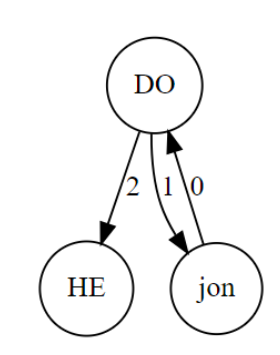
\includegraphics[scale=0.4]{figures/merge}
	\caption{Merged graph of answer candidate \textit{"Jon"} for the
		question \textit{Who did it?}}
	\label{fig:merge}
\end{figure}

\subsection{Experiments}
\label{sec:exp}

Demonstrating the algorithm behind my baseline, let's look at the example passage:
\begin{center}
	\textit{ "I went into my bedroom and flipped the light switch. Oh, I see that the ceiling lamp is not turning on. It must be that the light bulb needs replacement. I go through my closet and find a new light bulb that will fit this lamp and place it in my pocket. I also get my stepladder and place it under the lamp. I make sure the light switch is in the off position. I climb up the ladder and unscrew the old light bulb. I place the old bulb in my pocket and take out the new one. I then screw in the new bulb. I climb down the stepladder and place it back into the closet. I then throw out the old bulb into the recycling bin. I go back to my bedroom and turn on the light switch. I am happy to see that there is again light in my room."}
\end{center}
And a question related to the text: \textit{Which room did the light go out in?} and the answers:
\begin{itemize}
	\item \textit{"Kitchen."}
	\item \textit{"Bedroom."}
\end{itemize}
First the expanded graph from the text was built. After I constructed the merged graphs (for the demonstration, only the graphs without expansion was built) seen in Figure \ref{fig:merge1} and Figure \ref{fig:merge2}. The graph without merging can be seen in Figure \ref{fig:merge3}. After the merging, I compared both of the graphs to the passage graph applying my defined metric.

\begin{figure}
	\centering
	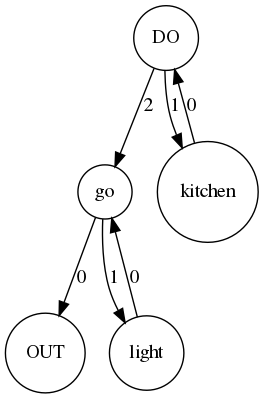
\includegraphics[scale=0.4]{figures/comp}
	\caption{Merged graph of answer candidate \textit{"Kitchen."}}
	\label{fig:merge1}
\end{figure}

\begin{figure}
	\centering
	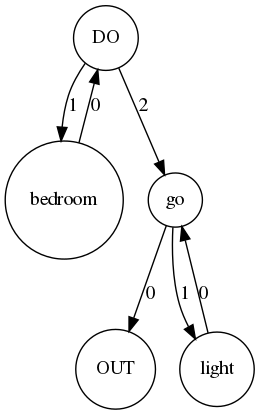
\includegraphics[scale=0.4]{figures/comp2}
	\caption{Merged graph of answer candidate \textit{"Bedroom."}}
	\label{fig:merge2}
\end{figure}

\begin{figure}
	\centering
	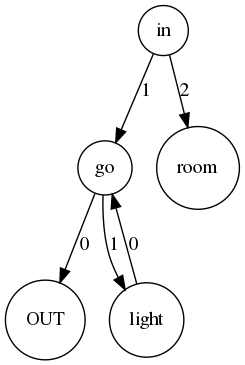
\includegraphics[scale=0.4]{figures/compdef}
	\caption{Graph built from the question}
	\label{fig:merge3}
\end{figure}

I tested the baseline method described in this section on a
subset of all questions in the train section of the MC dataset:
wh-questions that were not
categorized as "common-sense". Of this subset of 5,375 questions (of a
total of 9,731), our
method correctly answers 3,671, achieving an accuracy score of $68.3\%$.
I then proceeded to use the metric underlying our baseline as an
additional feature in the \texttt{Yuanfudao} system. 

In the next section I will briefly give an introduction into the field of deep learning in general, and particularly in NLP applications, and then I will demonstrate the Yuanfudao system.
%----------------------------------------------------------------------------
\section{Deep learning neural networks}
\label{sec:deep}

In this section I will introduce the basic deep learning related concepts necessary to understand the model described in the next section.

\subsection{Context}
With the recent increasing capabilities in computational power,
deep learning neural networks gained popularity again in recent years, after the AI winter ended. Since then neural networks became part of the everyday life, we hear about artificial intelligence being used in smart phones to enhance images quality or recognize certain settings and take a picture accordingly. AI is also being used in cancer research and other fields of bioinformatics, and personal assistants became extremely popular as well.

But even with the seemingly endless capabilities of artificial neural networks we are far from creating anything that could have the cognitive capacities of humans. This problem is considered by many to be AI-complete or AI-hard, meaning that creating a network that could keep up a human-like conversation would require data scientist and researchers to construct a universal artificial intelligence. A small but important step to achieve this is to create a system capable of doing simple reading comprehension tasks that also require some common sense knowledge.

The most common structures of these experimental neural networks include recurrent neural network layers and attention layers. Before the explanation of the function of these building-blocks, laying down the foundations is needed.

This section will introduce the essential deep learning mechanisms mainly used in NLP applications, and the main building blocks of the Yuanfudao system described in Section \ref{sec:yuanfudao}.

\subsection{Basics}
\begin{minipage}{\textwidth}
	Some arbitrary definitions this section uses:
	\begin{itemize}
		\item \textbf{Batch}: The chunks of training data that one iteration of the training uses. It's size can be a crucial parameter to set.
		\item \textbf{Epoch}: One training iteration is called an epoch. The number of epochs determines how long we want to train our network.
		\item \textbf{Learning rate}: \(\eta\) the velocity of the learning process. Setting it too low could result in slow learning and getting stuck in a local minimum, but setting it too high could result in jumping over the optimum and bouncing.
		\item \textbf{Accuracy}: The ratio of the correct predictions from all of the predictions. The goal of neural networks is to achieve high accuracy with on the test set.
		\item \textbf{Test set}: The part of the dataset that we don't use during the training of our neural network. This determines the actual accuracy of the network.
		\item \textbf{Training set}: The data that is used for training. The network is usually split into two parts with 80:20 ratio. We use the bigger set of data to train our network and we call this the training set.
		\item \textbf{Development set or Validation set}: The smaller portion of the data. We use this section to validate the network during its training. This section of the data shall not be used for training.
	\end{itemize}
\end{minipage}
\\
\\
People usually use supervised learning in the field of natural language processing to achieve the desired structure, but we might face multiple challenges while training. That's the reason why  optimization and regularization methods are needed.

\subsection{Optimization}
The goal of optimization is to overcome the following problems:
\begin{itemize}
	\item Local minimum
	\item Setting the learning rate
	\item Setting the batch size
\end{itemize}

We have touched on the first two briefly before, but setting the batch size is also very important. We give the training data to the network in batches, and we iterate through them multiple times (depending on the epoch).

Methods used for optimizing:
\begin{itemize}
	\item \textbf{Stochastic gradient descent}
	\item \textbf{Momentum}
	\item \textbf{Adaptive learning rate}
	\item \textbf{Adam} (Adaptive learning rate and momentum)
	\item \textbf{AdaMax} (Adam variant)
\end{itemize}

\paragraph*{Stochastic gradient descent}
\[g \leftarrow \frac{1}{batchSize}\Delta_w \sum_{i=1}^{batchSize}Loss(f_w(x_i), y_i)\]
Where f is the network itself.
\[w \leftarrow w - \eta g\]
This is a classical method for optimizing. It does not account for dynamic parameter settings. The system described in Section \ref{sec:yuanfudao} can use this function.
This is considered as our base, and only the differences between this and other optimization methods will be highlighted.

\paragraph*{Momentum}
\[g \leftarrow \alpha g + \frac{1}{batchSize}\Delta_w \sum_{i=1}^{batchSize}Loss(f_w(x_i), y_i)\]
Where \(\alpha\) is a parameter we can set.
This method has an added parameter, that helps taking into account the previous iterations, giving a momentum to the learning towards the optimum.

\paragraph*{Adaptive learning rate}
\[r \leftarrow r + g^2\]
Where r is a parameter that's initial value can be set.
\[w \leftarrow w - \frac{\eta}{\sqrt{r}} g\]
As the name suggests the adaptive learning rate uses a parametrization to slowly decrease the learning rate through time, depending on the previously calculated gradient.

\paragraph*{Adam}
\[r \leftarrow \varphi_r r + (1 - \varphi_r) g^2\]
\[s \leftarrow \varphi_s s + (1 - \varphi_s) g\]
Where s is a parameter that's initial value can be set and \(\varphi\) is a parameter of the decay rate.
\[w \leftarrow w - \frac{\eta s}{\sqrt{r}} g\]
Adam is one of the most popular optimizer function nowadays. It combines the adaptive learning rate and the momentum hence the name: Adam.

\paragraph*{AdaMax}
\[r \leftarrow \max(\varphi_r r, |g|)\]
\[s \leftarrow \varphi_s s + (1 - \varphi_s) g\]
\[w \leftarrow w - \frac{\eta}{1 - \varphi_s}\frac{s}{r}\]
A variant of the Adam optimizer. It was first described in the \textit{Adam: A method for stochastic optimization} article \cite{Kingma:2015}. It differs from Adam in that it uses a max operation and the infinity norm. The system described in Section \ref{sec:yuanfudao} can use this optimization function too.

\subsection{Regularization}
The goal of regularization is to avoid over-fitting. Over-fitting happens when our neural network produces good results on the training set's dedicated subset, the development or validation set, but it can't predict the expected outputs properly on a new dataset for example the test set. The network memorized the training set too much, and can function on that specific dataset only. It happens very often, so machine learning experts developed a couple functions to avoid this phenomenon.
\begin{itemize}
	\item \textbf{Weight decay}: Also known as L2 regularization. It uses a parameter to make sure that the previously learned weight won't influence the new one too much. \[w \leftarrow (1 - \eta \alpha)w - \eta \Delta_w Loss\]
	\item \textbf{L1 regularization}: This is a normalization method that modifies the cost function similarly to the L2 regularization. The difference is, that in this case the weights might get reduced to zero.
	\item \textbf{Dropout}: It randomly disables weights for an epoch, so they won't be used in that iteration.
	\item \textbf{Early stopping}: It stops the learning if the results on the development set haven't shown any progress in the last couple of epochs.
	\item \textbf{Noise injection}: It injects noise into the training set.
\end{itemize}

The system later described in Section \ref{sec:yuanfudao} uses dropouts while learning. This might cause the system's performance to fluctuate a little bit from epoch to epoch but it is a powerful tool for regularization and as we'll see later it manages to achieve consistently good results on the development set.

\subsection{Natural Language Processing with Deep learning}
As mentioned above the kind of layers used in Natural Language Processing are mostly recurrent neural network layers, attention layers and sometimes embedding layers.

\subsubsection{Embedding layers}

The function of embedding layers is to turn integer values to fixed length vectors, for example word embedding vectors discussed in Chapter \ref{chap:semanticparsing}. They are used mostly in natural language processing to work as word2vec translation.

When using embedding layers we want to find vectors for each word so that it can model the word's meaning. We achieve this by looking at the context the word usually appears in. If two words like \textit{apple} and \textit{orange} usually appear in the same context, than the vectors assigned to these words should have low cosine distance between them. It is explained in Chapter \ref{chap:semanticparsing}.

If you are building an NLP model, the embedding layer should be in the first layer, since its purpose is to make the transition from word to vector, and the word in this case is the input.

\begin{figure*}[!htb]
	\centering
	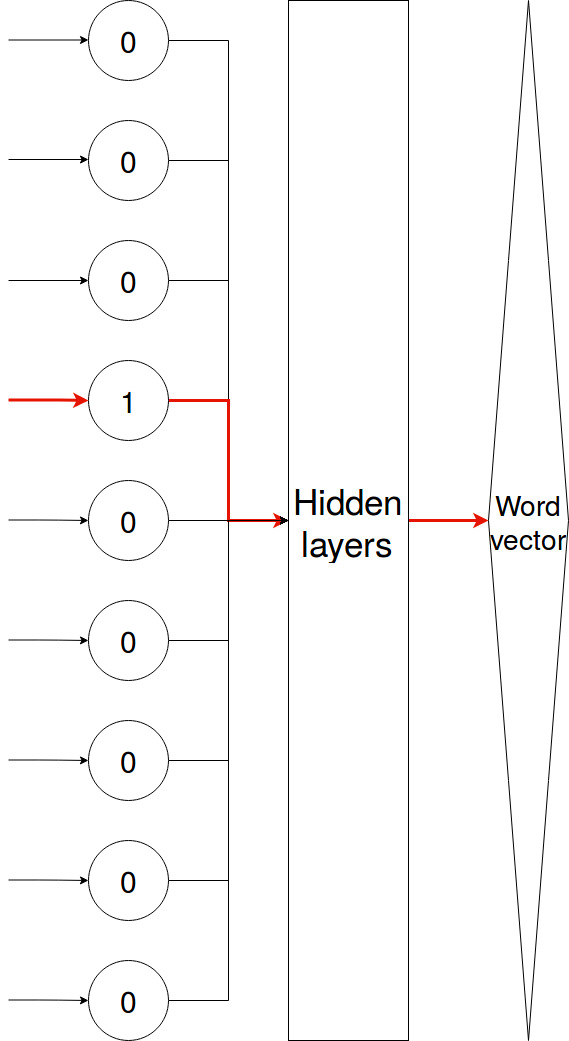
\includegraphics[scale=0.25]{figures/embedding_layer.jpg}
	\caption{An embedding layer.}
	\label{fig:embedding_layer}
\end{figure*}

The input dimension of this layer is the size of the vocabulary and the output dimension is the size of the dense vector. Usually the vocabulary size greatly exceeds the embedding dimension since the output vectors size is fixed and can range from 300 to 1000, and the vocabulary - depending on the dataset - can be way higher than that. See at Figure~\ref{fig:embedding_layer}.

They work mostly like a lookup table that can be trained. A lot of the times we use pretrained models, like the GloVe embeddings that have been trained on enormous datasets. We can also train them on our specific problem, or use the pretrained and our own embeddings simultaneously.
\FloatBarrier

\subsubsection{Recurrent Neural Networks}

In a simple feed forward neural network, the information only moves in one direction: from the input layer to the output layer. On the other hand recurrent neural networks take into account their immediate past, the output of the network with the previous timestamp. This internal "memory" like functionality allows the network to remember what it had calculated before. This is illustrated at Figure~\ref{fig:recurrent_net}.

At every timestamp the network gets two sets of inputs: the actual input at the timestamp and the hidden state of the network for the previous input. In one iteration it calculates its output using the calculated hidden state in the timestamp. It all could be imagined like the same feed forward network being repeated after one other.

The hidden state mentioned above is the "memory" of the network that is calculated with the previous hidden state and the input.

\begin{figure*}[!htb]
	\centering
	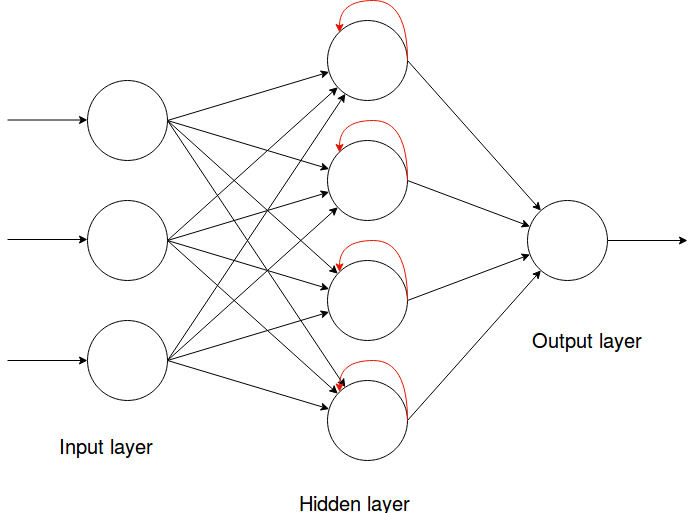
\includegraphics[scale=0.5]{figures/recurrent_neural_network.jpg}
	\caption{A recurrent neural network.}
	\label{fig:recurrent_net}
\end{figure*}

The backpropagation is also slightly different in this case, it's called backpropagation through time, you need to "unroll" the network (see at Figure~\ref{fig:unrolled}), and use the backpropagation starting from the right timestamps. Each timestamp's backpropagation could be understood as backpropagation on a separate feed forward neural network. 
\begin{figure*}[!htb]
	\centering
	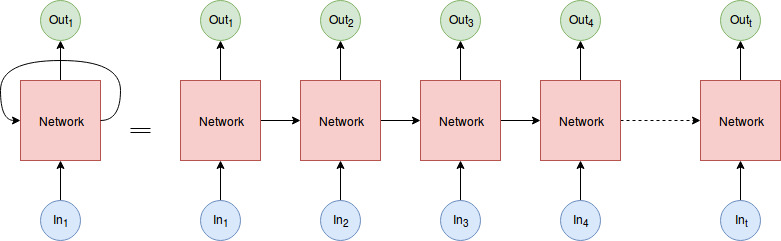
\includegraphics[scale=0.5]{figures/unrolled.jpg}
	\caption{Unrolled recurrent neural network.}
	\label{fig:unrolled}
\end{figure*}

The gradient vanishing or explosion can be a problem with this RNN.

There is a multitude of solutions for the exploding gradients, one of which is called gradient clipping. This is one of the method the state-of-the art system, Yuanfudao uses.

This technique is a very simple yet powerful way of dealing with exploding gradients. All it does is that it limits the size of the gradient, if its norm is higher than a set threshold.

RNNs can be used in supervised and also unsupervised learning. They are used when the data is sequential, like text, audio, etc.

\subsubsection{Long-Short Term Memory}
The system we worked with uses LSTM layers as its default RNN type.
Long-short term memory networks are the extension of the previously discussed recurrent neural network. The main difference is that it also has an internal long term memory. Usually these type of networks are more reluctant to have the exploding gradient problem.

Like the simple RNN, LSTMs also have hidden states, that are calculated slightly differently.
\\

\begin{minipage}{\textwidth}
	The LSTMs hidden states are calculated using three gates:
	\begin{itemize}
		\item \textbf{input gate}: determines whether to let new input in
		\item \textbf{forget gate}: determines whether to forget an input because it's not relevant anymore
		\item \textbf{output gate}: determines whether to let the input impact the output with the current timestamp
	\end{itemize}
\end{minipage}

These gates are analog and their values ranges from 0 to 1 with the sigmoid function. A simplified depiction can be seen at Figure~\ref{fig:lstm}\footnote{\url{https://en.wikipedia.org/wiki/Long_short-term_memory}}.
\begin{figure*}[!htb]
	\centering
	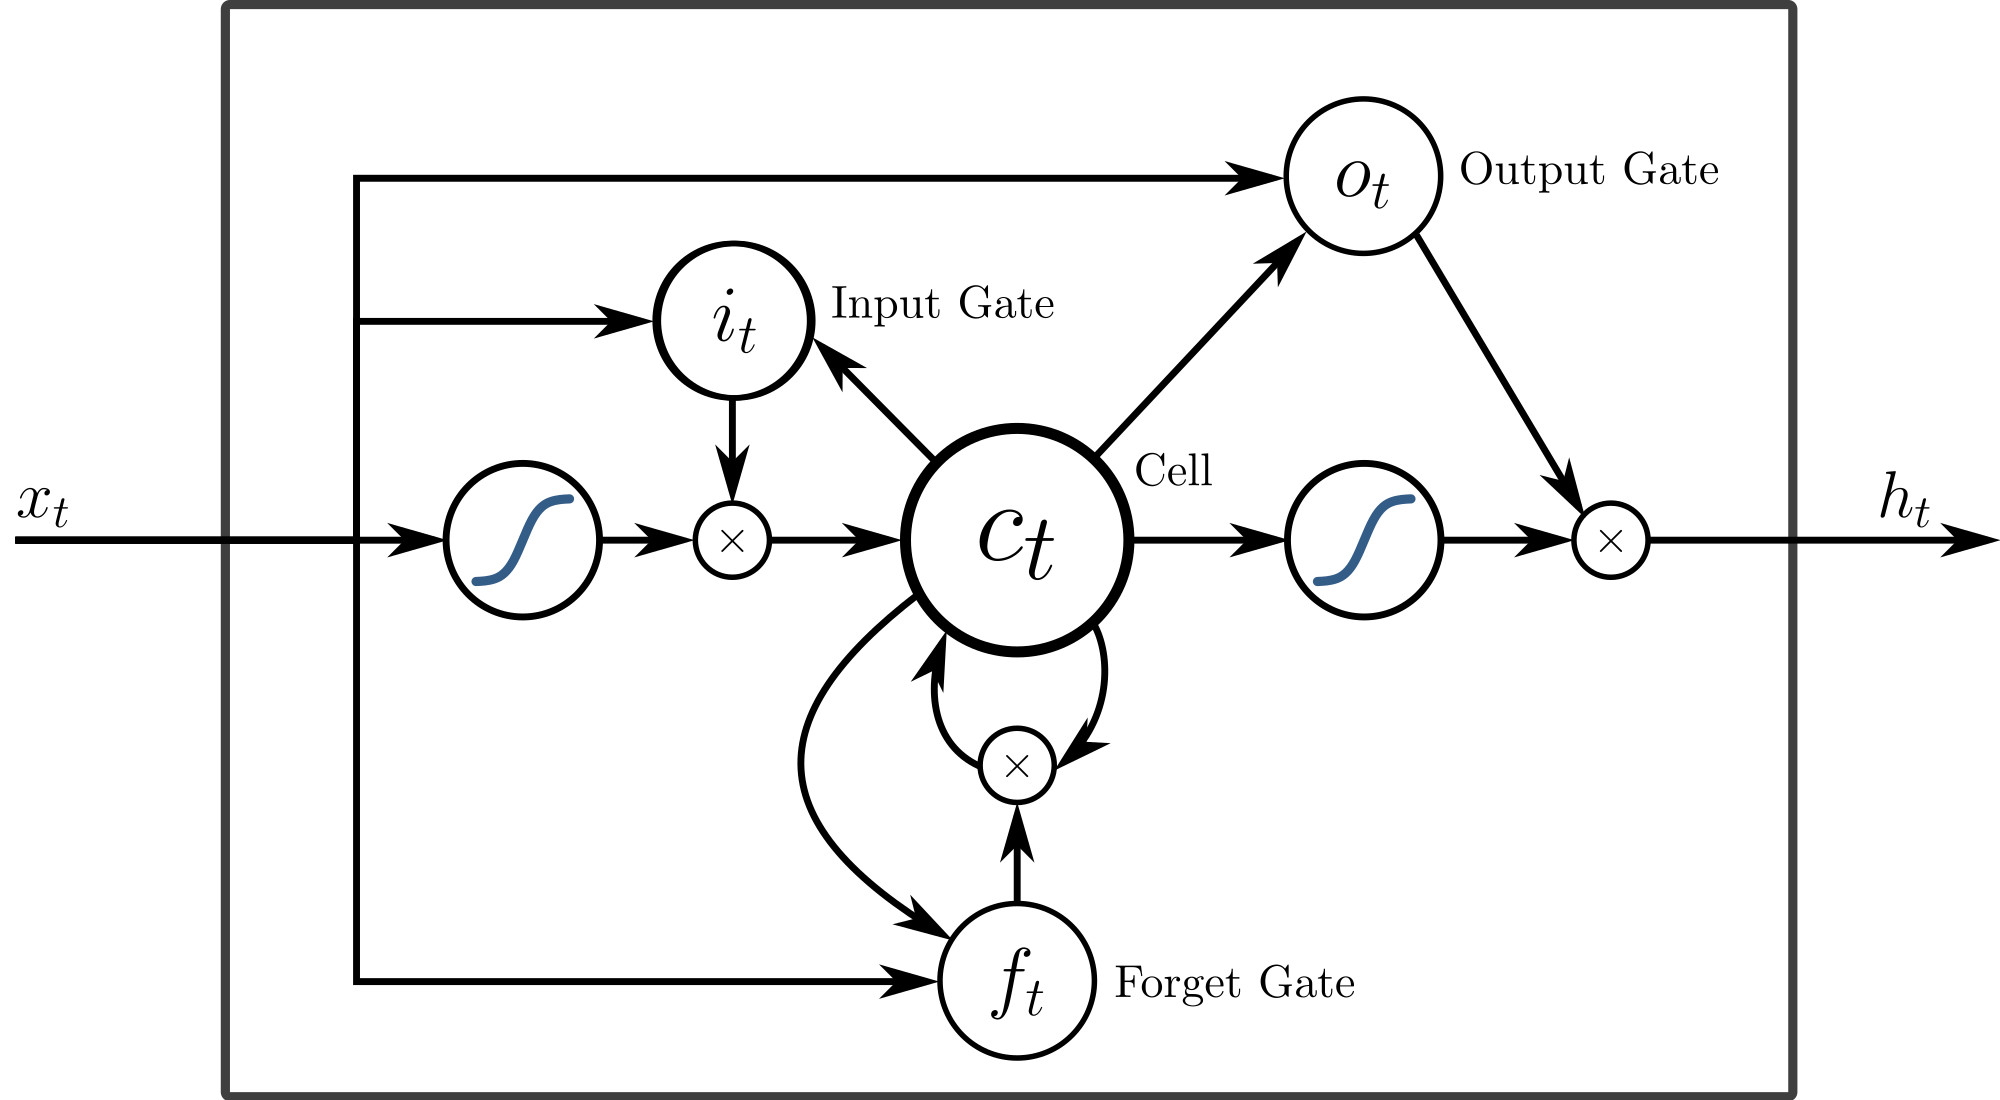
\includegraphics[scale=0.2]{figures/lstm.jpg}
	\caption{A long-short term memory network's gates.\\Image from Wikipedia}
	\label{fig:lstm}
\end{figure*}
\FloatBarrier

The sigmoid function allows this structure to be able to learn, meaning that we can use the backpropagation through time method described above.

Long-short term memory networks are used in natural language processing, but also in generative networks, like video or image description generation, text generation and so on.

\paragraph*{Bidirectional long-short term memory} also known as BiLSTM\\
BiLSTM networks are a variant of long-short term memory that read the input from the beginning to the end then also from the end to the beginning. The main idea behind this is that we may need not just the previous output, but also the next one too. These networks usually outperform simple LSTM systems in their predictions and the learning velocity too.

\subsubsection{Gated recurrent unit}
The system we worked with can use GRU layers as its RNN type, but it's not its default setting and it did not perform as good.
Gated recurrent units are also a type of RNN and have a similar structure (Figure~\ref{fig:gru}\footnote{\url{https://en.wikipedia.org/wiki/Gated_recurrent_unit}}) to the long-short term memory network, but has been shown to exhibit better performance on smaller datasets, than the LSTM.
\begin{figure*}[!htb]
	\centering
	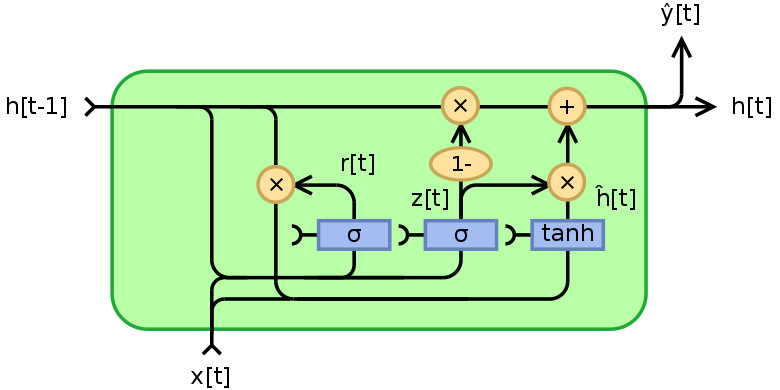
\includegraphics[scale=0.5]{figures/gru.jpg}
	\caption{A gated recurrent unit's gates.\\Image from Wikipedia}
	\label{fig:gru}
\end{figure*}

\begin{minipage}{\textwidth}
	It has four main building blocks:
	\begin{itemize}
		\item \textbf{update gate}: the gate gets the x[t] and the h[t-1] as its input and z[t] is the output on the image
		\item \textbf{reset gate}: the gate gets the x[t] and the h[t-1] as its input and r[t] is the output on the image
		\item \textbf{current memory content}: the gate gets the x[t], the h[t-1] and the r[t] as its input and \^{h}[t] is the output on the image
		\item \textbf{final memory at current time step}: the h[t] on the image
	\end{itemize}
\end{minipage}

Gated recurrent units are mostly used on the field of speech recognition and music modeling while the LSTM is more relevant on the field of natural language processing.

\subsubsection{Attention}
The Attention mechanism was first described in \cite{Bahdanau:2015} and was used for machine translation. Since then it became a widely used tool in natural language processing. The idea behind this mechanism is that when the neural network predicts the output, it only uses parts of the given input instead of the full input. That is where the most relevant information is concentrated and this mechanism only pays \textit{attention} to these parts and the network has to learn what to pay attention to.

Usually in the "sequence-to-sequence" tasks like MT there are two main parts of the model an encoder and a decoder. The encoder and the decoder are usually some type of RNN, mostly LSTM. The encoder is responsible for creating a so called context-vector from the input sequence. This context-vector has a fixed length and it serves as the representation of the sequence inside the model. The decoder then decodes this context-vector to a sequence again, in the case of the machine translation this sequence is in a different language. A depiction can be seen at Figure~\ref{fig:seq_to_seq}.
\begin{figure*}[!htb]
	\centering
	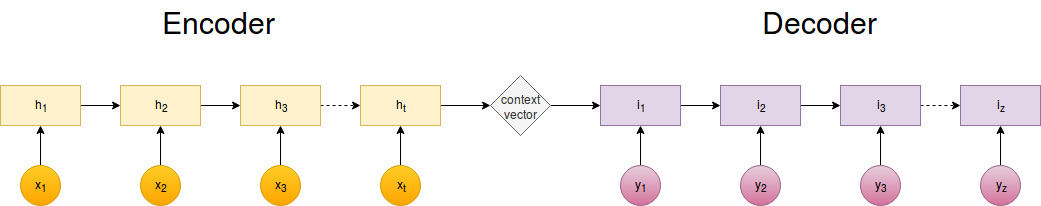
\includegraphics[scale=0.4]{figures/seq_to_seq.jpg}
	\caption{A sequence-to-sequence model with encoder and decoder.}
	\label{fig:seq_to_seq}
\end{figure*}

The attention mechanism described in \cite{Bahdanau:2015} was used in the decoder part of this model, the encoder functions the same way. The paper explicitly stated that this attention mechanism relieves the encoder from having to encode every sequence to a fixed length context vector. In this case we have a context vector for every word of the expected output. These context-vectors are the weighted sums of the encoder's states (\textit{annotations}).
\[c_i = \sum_{j=1}^{t} \alpha_ij h_j\]
Where \(\alpha\) parameter is calculated like the following:
\[\alpha_ij = \frac{exp(e_{ij})}{\sum_{k=1}^{t} e_{ik}} \]
and \(e_{ij}\) is its energy
\[e_{ij} = a(s_{i-i}, h_j)\]
This is an \textit{alignment model} that scores how well the input around \textit{j} and the output around \textit{i} match. This \textit{alignment model} is a feed forward neural network that is trained simultaneously with the other components of the system.
The decoder uses the previous state's output and its assigned context-vector when calculating its own target.
\[s_i = f(s_{i-1}, y_{i-1}, c_i)\]
The attention based model is at Figure~\ref{fig:attention}.
\begin{figure*}[!htb]
	\centering
	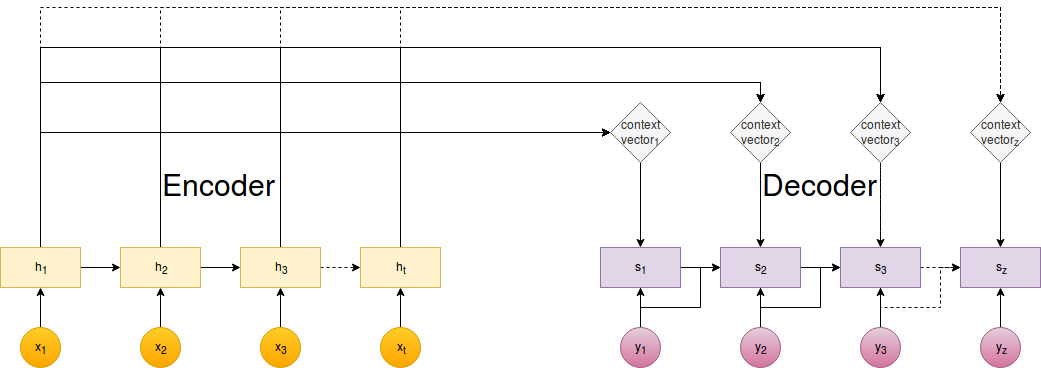
\includegraphics[scale=0.4]{figures/attention.jpg}
	\caption{A sequence-to-sequence model with encoder-decoder and attention.}
	\label{fig:attention}
\end{figure*}

A big advantage of using this mechanism is the ability to interpret our model. These days it's more important than ever to be able to tell why does the network predict what it predicts, and thanks to the attention mechanism we are able to say that (in a purely attention-based network). One example is shown at Figure~\ref{fig:interpretation}.

\begin{figure*}[!htb]
	\centering
	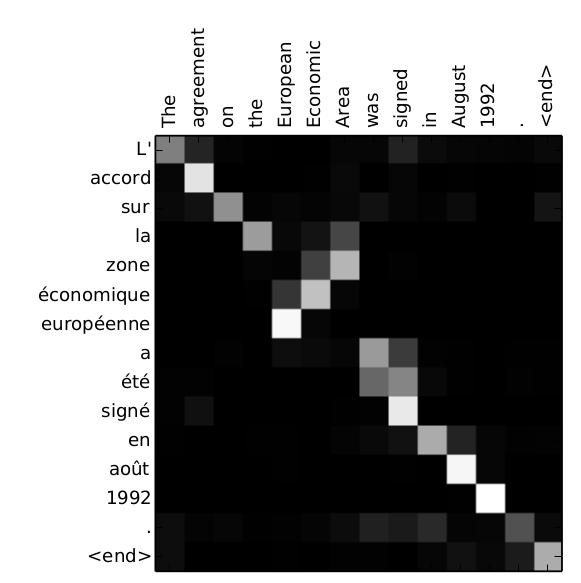
\includegraphics[scale=0.5]{figures/interpretation.jpg}
	\caption{An interpretation of a french - english sequence to sequence translation.\\Image from \cite{Bahdanau:2015}.}
	\label{fig:interpretation}
\end{figure*}

\begin{minipage}{\linewidth}
	Since its first description in \cite{Bahdanau:2015} the attention mechanism has been used for:
	\begin{itemize}
		\item \textbf{Image caption/description}: a convolutional neural network translates the image to the context vectors and the decoder creates a description for it. A recent system using attentions for image captioning is described in the \textit{Image Caption with Global-Local Attention} paper \cite{Li:2017c}.
		\item \textbf{Grammar representation}: in this case the decoder builds a grammatical representation for the input. On a related field there was a study regarding linguistic representations and attentions \cite{Kadar:2016}.
		\item \textbf{Advanced machine translation}: Since it was first introduced it has revolutionized the field of machine translation. A study on this field is \textit{Effective Approaches to Attention-based Neural Machine Translation} \cite{Luong:2015b}.
		\item \textbf{Machine comprehension tasks}: question answering based on a previously read text. The system described in Section \ref{sec:yuanfudao} is like this \cite{Wang:2018}.
	\end{itemize}
\end{minipage}
%----------------------------------------------------------------------------
\section{Yuanfudao system}
\label{sec:yuanfudao}
On the 2018 Semeval Task \textit{Machine comprehension using commonsense knowledge} competition the \texttt{Yuanfudao} \cite{Wang:2018} system reached second place with $83.95\%$ accuracy on the test data.

% Yuanfudao introduction
\subsection{The original system}

The \texttt{Yuanfudao} system implements a Three-way Attentive Network (TriAN), an ensemble of three LSTMs augmented with various attention mechanisms, to model for each question interactions between question, possible answers, and the passage that may or may not contain the correct answer to the question.

The system was implemented using python programming language and the \texttt{pytorch} package for the implementation of the neural network. The source code is available on Github\footnote{\url{https://github.com/intfloat/commonsense-rc}}.

% Yuanfudao preprocess

\subsection{Preprocessing}
This system processes the input data as follows:

\begin{enumerate}
	\item Using the \texttt{spacy} package's tokenizer function it generates the part of speech (pos) tag, named entity recognition (ner) tag and the lemma for each word in the passage, and the pos tags of the questions.
	\item It assigns a number representation and an offset for each word in the passage, questions and answers.
	\item It also saves the ids of the passages, questions and answers and whether the answer was correct.
	\item The preprocessor finds the words and lemmas in the questions and answers, that also occurred in the passage's word and lemma list. 
	\item It stores each word's frequency using the \texttt{wikiwords} library.
	\item It  establishes the \textit{ConceptNet} relation between the words of the passage and question and also between the words of the passage and answer.
	\item The preprocessor saves all this data to their respective json files.
\end{enumerate}


\paragraph*{Conceptnet} \cite{Speer:2017} \\

\textit{ConceptNet} plays a major part of the \texttt{Yuanfudao} system, as it was shown in the original paper \cite{Wang:2018}. This is a metric  used to show the possible relationship between two words. These relations could be "RelatedTo", "IsA", "Synonym", "PartOf" etc. 

The \textit{ConceptNet} itself is a large graph of general knowledge that has shown to be affective at determining word relations.

The preprocessor compares the words in the passage with the words in the "query" (question or answer) using \textit{ConceptNet} and stores only one of the matches per word, if there were any.

% System description

\subsection{System description}

An overview of the original system is reproduced in Figure~\ref{fig:dnn}.
\begin{figure}[h!]
	\centering
	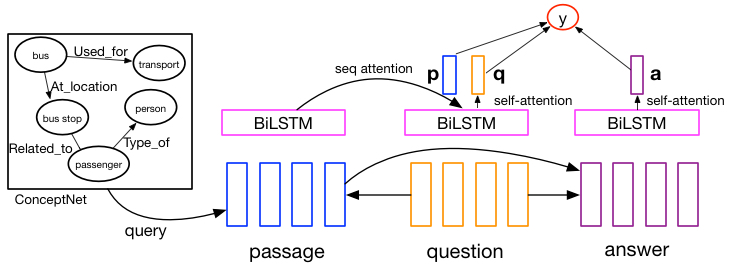
\includegraphics[scale=0.5]{figures/TriAN.jpg}
	\caption{Structure of the original network \cite{Wang:2018}}
	\label{fig:dnn}
\end{figure}

This system is a deep learning neural network consisting of embeddings, recurrent neural networks and attention mechanisms.

First the inputs generated in the preprocessing phase go through three embedding layers, each corresponding to the passage, question and answer respectively. There are also pos-embedding, ner-embedding and rel-embedding layers. The pos-embedding gets the passage's and the question's pos tags as its input, the ner-embedding layer gets the passage's ner-tags and the relation-embedding gets the relationship vectors generated using the \textit{ConceptNet}. This input embedding layer is shown in Figure~\ref{fig:embedding}.
\begin{figure}[h!]
	\centering
	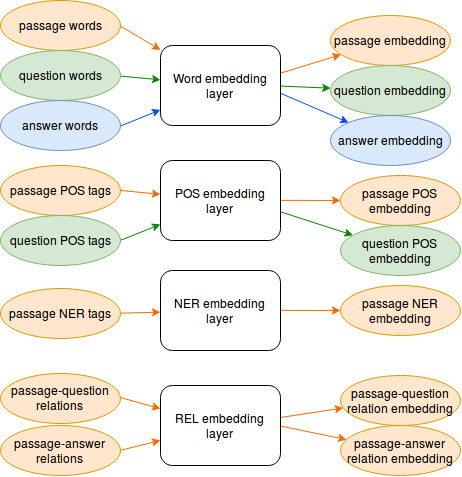
\includegraphics[scale=0.5]{figures/TriAN_embeddings.jpg}
	\caption{Structure of the input embedding layers.}
	\label{fig:embedding}
\end{figure}

The word embeddings' outputs are paired up (passage-question, answer-question, answer-passage) and go through a so called \textit{sequence attention matching layer}.
The sequence attention matching layer at its core uses the bmm function in \texttt{pytorch} which performs a batch matrix-matrix product of the input matrices.
This way it "matches" the two inputs together. This is shown in Figure~\ref{fig:attention_match}.
\begin{figure}[h!]
	\centering
	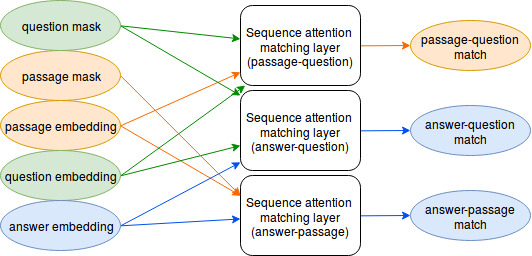
\includegraphics[scale=0.5]{figures/TriAN_attention_match.jpg}
	\caption{Structure of the \textit{sequence attention matching layers}.}
	\label{fig:attention_match}
\end{figure}

The system uses dropouts after the embedding and sequence attention matching layers to avoid over-fitting.

These layers are followed by three \textit{stacked bidirectional RNN layer}, each corresponding to the passage, question and answer respectively. It differs from the standard bidirectional RNN layer in one aspect: it can concatenate the hidden states of the RNN. By default the type of the RNN is LSTM, but it can also be GRU. Their inputs are sort of self explanatory. The passage's stacked bidirectional RNN layer gets the passage's word embedding layer, the output of the sequence attention matching layer for the passage-question input pair, the passage's pos- and ner-embedding layers, the word frequency tensor created with the \texttt{wikiword} library, and the two relation-embedding layer's output. The question's stacked bidirectional RNN layer expects the question's word and pos-embedding outputs on its input. The answer's stacked bidirectional RNN layer's inputs are the answer's word embedding output and  the output of the sequence attention matching layer for the answer-question and the answer-question input pairs. These RNN layers are shown in the Figure~\ref{fig:rnn}.
\begin{figure}[h!]
	\centering
	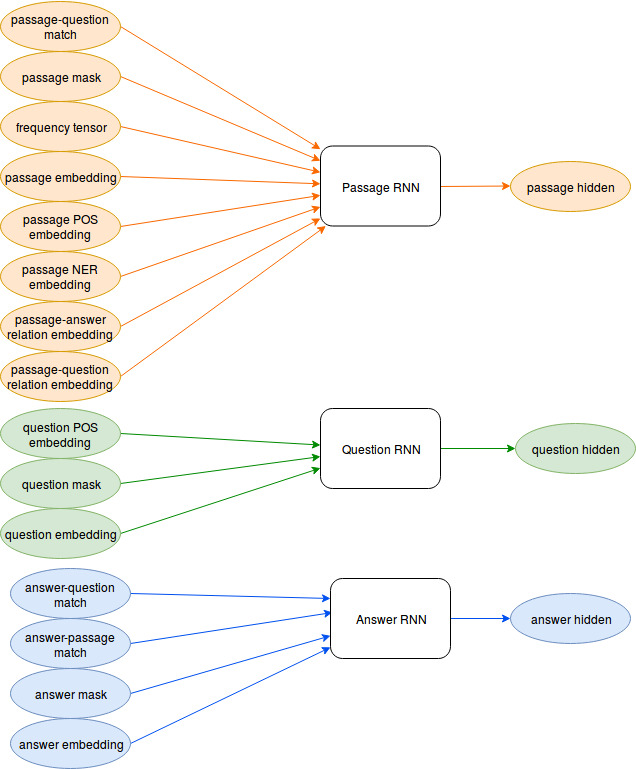
\includegraphics[scale=0.4]{figures/TriAN_rnn.jpg}
	\caption{Structure of the \textit{stacked bidirectional RNN layers}.}
	\label{fig:rnn}
\end{figure}
This layer implicitly uses a dropout rate for regularization.

The question's and the answer's stacked bidirectional RNN layer's outputs are used in two \textit{linear sequence attention layers}, or better known as \textit{self-attention layers over a sequence} for the question and the answer respectively. This layer is basically a linear layer slightly modified, so the infinite outputs are masked and it uses a softmax function at its output.

The passage's stacked bidirectional RNN layer's output is used differently. The system passes it and the question's \textit{stacked bidirectional RNN layer's} output to a \textit{bilinear sequence attention layer}, which is similarly to the sequence attention matching layer uses the bmm function as its core function.

The two linear sequence attention layer's and the bilinear sequence attention layer's output is passed through a weighted averaging function with their respective stacked bidirectional RNN layer's output. This part of the network is shown in Figure~\ref{fig:sequence_attention}.
\begin{figure}[h!]
	\centering
	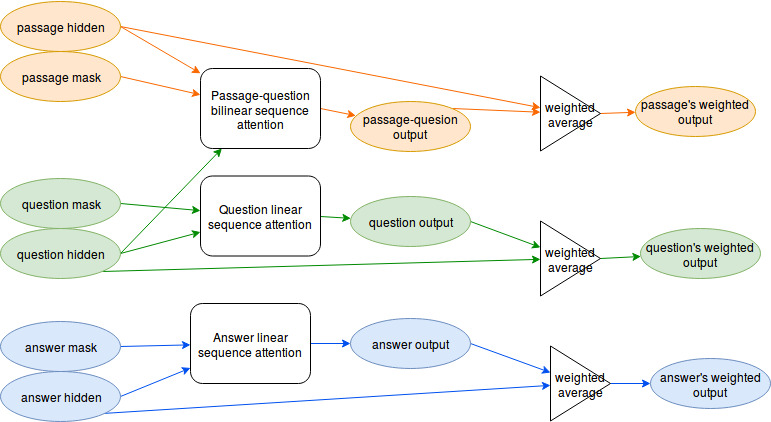
\includegraphics[scale=0.5]{figures/TriAN_sequence_attention.jpg}
	\caption{Structure of the sequence attention layer\\and the following weighted average function.}
	\label{fig:sequence_attention}
\end{figure}

The averaged passage output is passed through a \textit{linear feed forward layer} then multiplied by the answer's averaged output. The question's averaged output is passed through an other linear feed forward layer than multiplied by the answer's averaged output. At the end its all summed and sigmoid function used at its output. The output in this case is whether the answer was correct to the given question or not. This last section is at Figure~\ref{fig:output}.
\begin{figure}[!htb]
	\centering
	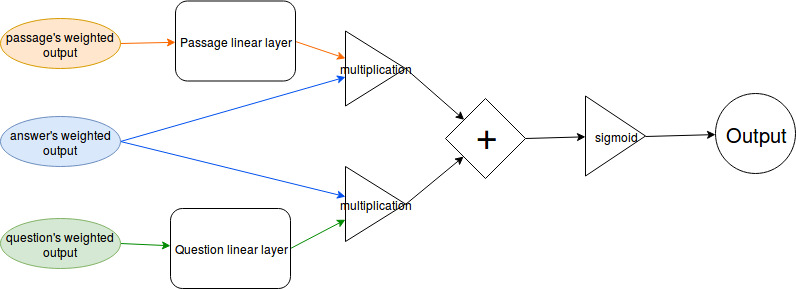
\includegraphics[scale=0.5]{figures/TriAN_output.jpg}
	\caption{Structure of the output of the network.}
	\label{fig:output}
\end{figure}


\subsection{Parameters}
\begin{minipage}{\textwidth}
	The \texttt{Yuanfudao} system has these following command line arguments:
	\begin{itemize}
		\item \textbf{GPU}: the training of the system can be done on GPU which is much faster than training it on CPU
		\item \textbf{using cuda}: \texttt{pytorch} can support CUDA for parallelization. The system uses CUDA by default.
		\item \textbf{optimizer}: the optimizer function can be adamax (default) or SGD
		\item \textbf{RNN type}: the RNN used by the system can be LSTM or GRU
		\item \textbf{dropout rate}: there are separate dropout rates for embeddings and RNNs
		\item \textbf{embedding dimension}: each embedding dimension in the system can be manually set
		\item \textbf{gradient clipping}: the gradient clipping threshold can be set
		\item \textbf{epoch}
		\item \textbf{learning rate}
		\item \textbf{batch size}
		\item \textbf{random seed}
		\item other parameters related to input handling, RNN settings and testing
	\end{itemize}
	You can read about the deep learning related arguments and their functions in Section \ref{sec:deep}.
\end{minipage}

\subsection{Learning curve}
\begin{minipage}{\linewidth}
	Without the recommended pretraining (Figure~\ref{fig:learning_curve}):
	\begin{itemize}
		\item Max dev accuracy: $82.7\%$ reached in the 26th epoch
		\item Train accuracy: $97.7\%$ reached in the 26th epoch
		\item Max train accuracy: $99.8\%$ reached in the 50th epoch
		\item Last dev accuracy: $81.9\%$
		\item Average dev accuracy after ten epochs: $81.9\%$
	\end{itemize}
\end{minipage}
\begin{figure}[!htb]
	\centering
	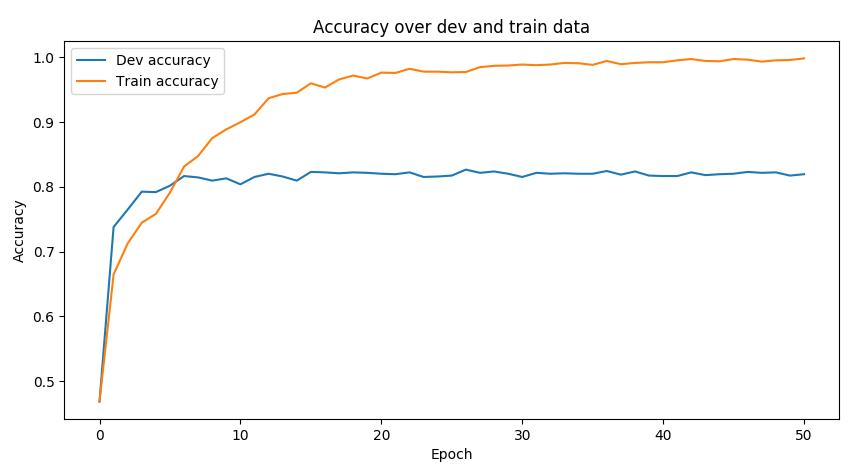
\includegraphics[scale=0.5]{figures/learning_curve.jpg}
	\caption{Learning curve without pretraining.}
	\label{fig:learning_curve}
\end{figure}

\begin{minipage}{\linewidth}
	With the recommended pretraining(Figure~\ref{fig:learning_curve2}):
	\begin{itemize}
		\item Max dev accuracy: $82.5\%$ reached in the 38th epoch
		\item Train accuracy: $99\%$ reached in the 38th epoch
		\item Max train accuracy: $99.7\%$ reached in the 50th epoch
		\item Last dev accuracy: $82.2\%$
		\item Average dev accuracy after ten epochs: $81.9\%$
	\end{itemize}
\end{minipage}
\begin{figure}[!htb]
	\centering
	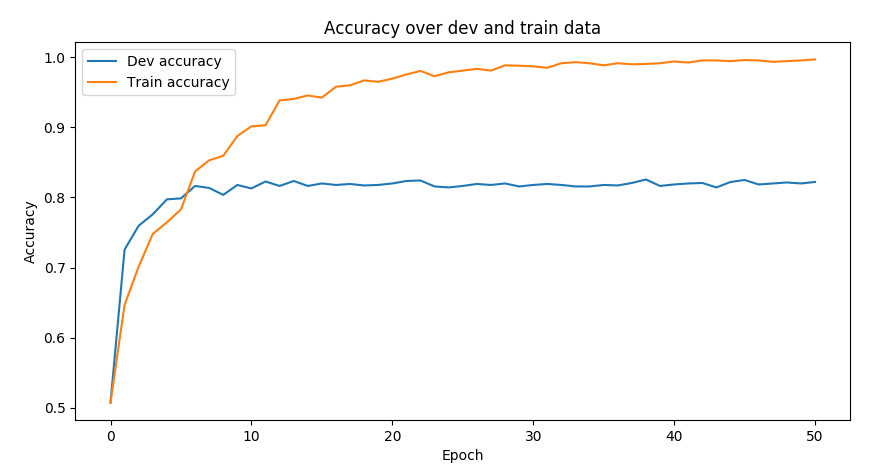
\includegraphics[scale=0.5]{figures/learning_curve2.jpg}
	\caption{Learning curve with pretraining.}
	\label{fig:learning_curve2}
\end{figure}

As you can see there is no significant difference between the learning curve with or without pretraining.

\section{Modifications}
Our modifications are available on Github\footnote{\url{https://github.com/GKingA/commonsense-rc}}.

We modified the preprocessing part of the system to incorporate the similarity calculating method from Chapter ~\ref{chap:comprehension}. The most straightforward way of incorporating our metric into the system is by creating vectors similar to those representing \textit{ConceptNet} relations between words of a passage and words in each answer candidate. Since these vectors represent
word-to-word relationships, we measure the support between pairs of \texttt{4lang} definition graphs, and for each word in the passage we take the maximum support score over all words of the answer candidate. Elements of a vector for a passage $P$ and a possible answer $A$ are hence defined as:

\[S^{(P, A)}_i = \max_{A_j \in A} S(P_i, A_j)\]

Elements of a vector for a passage $P$ and a question $Q$ are defined as:

\[S^{(P, Q)}_i = \max_{Q_j \in Q} S(P_i, Q_j)\]

Elements of a vector for a question $Q$ and an answer $A$ are defined as:

\[S^{(Q, A)}_i = \max_{A_j \in A} S(Q_i, A_j)\]

We used these new input vectors as the input of a new \texttt{4lang} embedding layer that functions similarly to the other embedding layers. It is shown at Figure~\ref{fig:4lang_embedding}. The input of this layer is 101 dimensional, since the similarities are on a scale to 0 to 100.

\begin{figure}[h!]
	\centering
	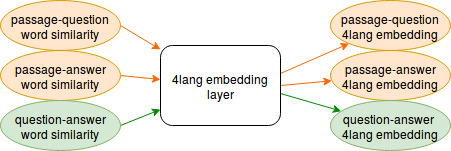
\includegraphics[scale=0.5]{figures/4lang_embedding.jpg}
	\caption{\texttt{4lang} embedding layer.}
	\label{fig:4lang_embedding}
\end{figure}

The outputs of this layer are passed to the RNN layers. This is depicted at Figure~\ref{fig:rnn_4lang}.

\begin{figure}[h!]
	\centering
	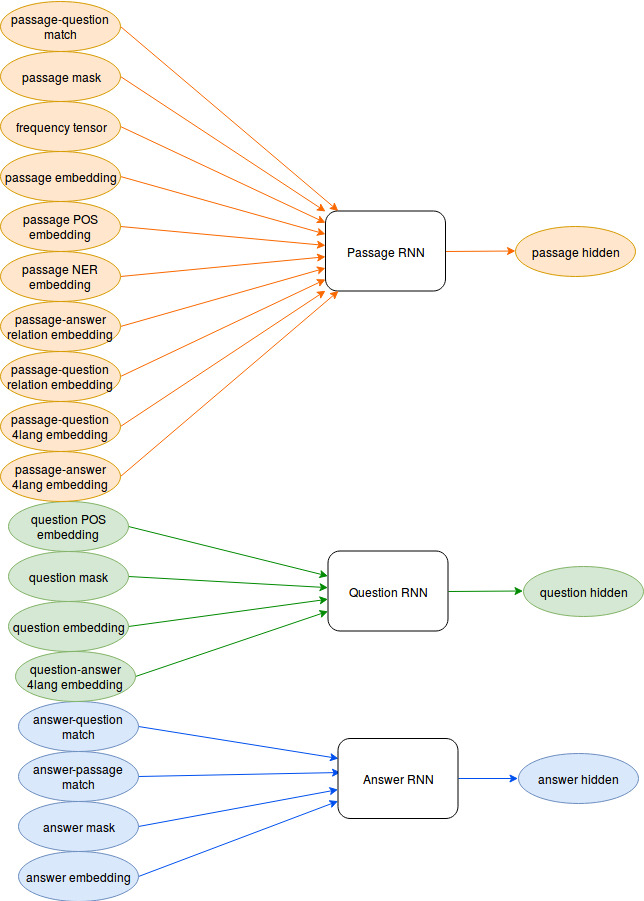
\includegraphics[scale=0.4]{figures/TriAN_rnn_with_4lang.jpg}
	\caption{Structure of the modified \textit{stacked bidirectional RNN layers}.}
	\label{fig:rnn_4lang}
\end{figure}

Since we also wanted to see how the system changes if we replace \textit{ConceptNet} relations with our metric, we also trained systems without \textit{ConceptNet} rel-embeddings.

\FloatBarrier

\section{The results}
The original \texttt{Yuanfudao} \cite{Wang:2018} publication said its system was able to reach $83.95\%$ accuracy on the test data. We were only able to reproduce a $80.3\%$ accuracy on the test set and $82.5\%$ on the development set with the recommended pretraining on the \texttt{RACE} \cite{Lai:2017} dataset. We will take these results as our bases of the comparison.

We tested our model by turning on and off the usage of \textit{ConceptNet} and \texttt{4lang}. There were 4 combinations: using neither, just \textit{ConceptNet}, just \texttt{4lang} and both.

\begin{table}[h!]
	\centering
	\begin{tabular}{ | l | c | r | }
		\hline
		model & dev & test \\ \hline \hline
		pretrained TriAN, no ConceptNet & 83.7\% & 81.9\% \\ \hline
		pretrained TriAN, with ConceptNet & 82.5\% & 80.3\% \\ \hline
		pretrained TriAN, with 4lang & 84.2\% & 81.5\% \\ \hline
		\textbf{pretrained TriAN, with both} & \textbf{83.4\%} & \textbf{82.9\%} \\ \hline
		TriAN, no ConceptNet & 82.8\% & 80.2\% \\ \hline
		TriAN, with ConceptNet & 82.7\% & 80.5\% \\ \hline
		TriAN, with 4lang & 83.2\% & 80.9\% \\ \hline
		TriAN, with both & 83.1\% & 80.8\% \\ \hline
	\end{tabular}
	\caption{Effect of \texttt{4lang} and \texttt{ConceptNet} on results}
	\label{tabl:res}
\end{table}

It is evident that without pretraining the Yuanfudao system performs best if we use the relation scores calculated from \texttt{4lang} graphs instead of the \textit{ConceptNet} relationships.
After pretraining the network on the \texttt{RACE} dataset the results show that using both of the relation metric is the most beneficial.
\chapter{Conclusion and future work}
\label{chap:future}

\section{Summary}
This thesis proposes a novel method for recognizing entailment using semantic
graphs and apply it to the 2018 Semeval task on Machine
Comprehension (MC). First, a brief overview of the field of natural language processing is given focusing on real life applications, that are in need of the NLP technologies. Then the topic of computational semantics was discussed in details, focusing on one-two major tasks, like question-answering or information retrieval. After that the formalism of 4lang was presented with examples, and the method of expansion was discussed. After simple yet a strong baseline method was presented for measuring
textual entailment and its application to the comprehension task, followed by an introduction to the field of deep learning. Finally the last chapter reports the results of applying the baseline method
to the MC task and also of using it as an extra feature in the neural network
based \texttt{Yuanfudao} system.

\section{Future work}
Our results are quite promising, but
further experiments are required to explore whether our enhancements can
improve the top-ranking system that also employs
pretraining and an ensemble of multiple models.
We also plan to incorporate sentence-level support
into the system as a more direct application of our
baseline. 

\subsection{Interpreted Regular Tree Grammar}
We recently started experimenting with Interpreted Regular Tree Grammars \cite{Koller:2011} (IRTG) that we could also use to construct \textbf{4lang} graphs, since they implement graph transformations, so graph grammars can be used. And by modifying the rules of the grammar, we can also accomplish the \textit{expand} functionalities and we also can define inference rules. These experiments are not yet perfect, but this approach shows great potential. See the phrase \textit{"Ordinary email"} represented in Figure~\ref{fig:irtg}.

The base of this approach is to define grammar files where we describe the rules using multiple graph, tree or string algebras. This allows us to use it as a graph rewriting grammar file which we can use to transcribe for example a universal dependency graph to a \texttt{4lang} graph.

We used an already functioning grammar that defined the relationships between universal dependencies and \texttt{4lang} graphs and modified it to incorporate the definition of the words also \cite{AcsEvelin:2018}.

\begin{figure*}[h]
	\centering
	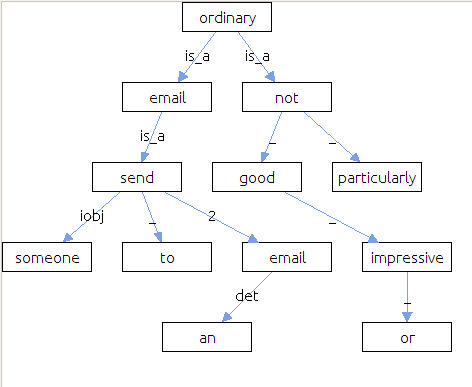
\includegraphics[scale=0.4]{figures/irtg.jpg}
	\caption{Example of the \textit{"expand"} method using IRTG}
	\label{fig:irtg}
\end{figure*}
%----------------------------------------------------------------------------
\chapter*{Acknowledgement}\addcontentsline{toc}{chapter}{Acknowledgement}
%----------------------------------------------------------------------------
First of all, 
I would like to express my deep gratitude to Dr. Recski G�bor for his guidance not just through this thesis, but through my whole master studies. I would like to thank him for introducing me to this interesting and amazing research field. He was always flexible and available for all my questions. I thank him for his valuable advices just about any topic imaginable.  

I am also thankful to Dr. Kornai Andr�s for his constant support
and help with my work. I thank him for his energy to discuss any of problems I have.

I also would like to thank to my colleague G�mes Kinga for her excellent work. 

Finally, a special thanks to my girlfriend for her constant love and support. I thank her for her supporting me even through difficult situations. Without her, I would not have been able to write this thesis.

\listoffigures\addcontentsline{toc}{chapter}{List of figures}
\listoftables\addcontentsline{toc}{chapter}{List of tables}

\bibliography{mybib}
\addcontentsline{toc}{chapter}{Bibliography}
\bibliographystyle{plain}

\label{page:last}
\end{document}
